\documentclass[a4paper,fleqn]{cas-dc}

\usepackage[numbers,sort&compress]{natbib}
\usepackage{amsmath,amssymb,amsfonts}
\usepackage{graphicx}
\usepackage{booktabs}
\usepackage{multirow}
\usepackage{xcolor}
\usepackage{hyperref}
\usepackage{listings}
\usepackage{subcaption}
\usepackage{array}
\usepackage{tabularx}

% Custom macros for exact empirical constants from the frozen Number Bank
% (paper/CEA Paper/manuscript/NUMBER_BANK.md -- every value below traces there).
\newcommand{\Nmisbind}{10{,}000}
\newcommand{\Nslots}{11}
\newcommand{\MisbindDetRate}{100.0\%}
\newcommand{\DetAdvisoryCoverage}{51.04\%}
\newcommand{\SafetyRefusalHandling}{10.48\%}
\newcommand{\LLMDependent}{38.48\%}
\newcommand{\LatencySpeedup}{2.28\times}
\newcommand{\SearchSpaceRedPct}{75.64\%}
\newcommand{\DialectHitAdvantage}{+36.6\,\text{pp}}
\newcommand{\SMSFidelity}{100.0\%}
\newcommand{\SMSHazardLLM}{64.4\%}
\newcommand{\TamperDetRate}{100.0\%}
\newcommand{\HumanGwetAC}{0.862}

\begin{document}
\let\WriteBookmarks\relax
\def\floatpagepagefraction{1}
\def\textpagefraction{.001}

% Short title and author running heads
\shorttitle{Bounded-Authority Agricultural Advisory}
\shortauthors{R. Reza et al.}

\title [mode = title]{Bounded-Authority Agricultural Advisory: Selective Resolution and Evidence-Bound Verification for Safe Bengali Decision Support}

\author[1]{Raiyaan Reza}[type=editor,auid=000,bioid=1,orcid=0009-0002-8610-8673]
\cormark[1]
\ead{raiyaan.reza@northsouth.edu}
\credit{Conceptualization, Methodology, Software, Formal Analysis, Writing - Original Draft, Project Administration}

\author[1]{Research Collaborator}[orcid=0000-0000-0000-0000]
\ead{collaborator@northsouth.edu}
\credit{Investigation, Data Curation, Validation, Writing - Review \& Editing}

\address[1]{Department of Electrical and Computer Engineering, North South University, Dhaka 1229, Bangladesh}

\cortext[cor1]{Corresponding author}

\begin{abstract}
Large Language Models (LLMs) and standard Retrieval-Augmented Generation (RAG) pipelines can be fluent and productive in multilingual agricultural extension, but generative models carry no intrinsic bound on factual authority. In safety-critical crop protection, a fluent sentence can silently misbind a pesticide to the wrong pest, inflate a dosage, confuse a formulation, or drop a mandatory Pre-Harvest Interval (PHI). This paper presents the \textbf{Bounded-Authority Advisory Architecture (BAA)}, an agricultural decision-support architecture that separates factual authority from linguistic realization. BAA enforces a fail-closed certification contract over structured, provenance-carrying evidence records and selectively routes each farmer query among deterministic resolution, grounded generation, conversational clarification, safe abstention, and expert escalation.

We evaluate BAA across an evidence chain that isolates each architectural decision. On 10,000 adversarial relational-misbinding attacks and 2,000 counterfactual evidence mutations, BAA rejects \MisbindDetRate{} of corrupted chemical claims (95\% Wilson CI [99.96\%, 100.0\%]), against 80.0\% dangerous acceptance for a lexical baseline and 38.65\% for an LLM-as-a-judge verifier. On a 100-case live end-to-end benchmark, BAA attains 97.0\% certified advisory correctness and 0.0\% critical unsafe acceptance (CI [0.0\%, 3.7\%]), with 33.0\% safe abstention; a three-agronomist validation study records a mean correctness rating of 4.82/5 and a 100.0\% chemical-safety pass rate (Gwet's AC1 = 0.862). Calibrated abstention sustains 84.56\% advisory coverage at a 1.26\% selective-risk level on 20,112 held-out cases. A five-tier resolution ladder resolves \DetAdvisoryCoverage{} of the modeled workload without invoking any LLM (safety/refusal handling \SafetyRefusalHandling{}, LLM-dependent traffic \LLMDependent{}), cutting weighted latency 2.28$\times$. Deterministic 160-character GSM templates preserve 100\% of safety-critical slots where LLM-composed SMS loses the PHI in 64.4\% of messages, and offline-first cryptographic caching sustains 91.4\% delivery at 15\% packet loss versus 82.0\% for cloud-only RAG. The results show that subordinating generative language to explicit, bounded factual authority yields a dependable, auditable, and affordable foundation for agricultural decision support in low-resource environments.

\end{abstract}

\begin{keywords}
Agricultural decision support \sep Large language models \sep Retrieval-augmented generation \sep Safety-critical verification \sep Bounded factual authority \sep Selective resolution \sep Low-resource NLP \sep Edge computing
\end{keywords}

\maketitle

% Include modular section files
\section{Introduction}
\label{sec:introduction}

\subsection{Agricultural Advisory as a Safety-Critical Computing Challenge}
Smallholder agriculture in low- and middle-income countries (LMICs) faces escalating pest and disease pressures driven by climate volatility, intensive cropping patterns, and fragmented extension services \citep{edgeagri2025}. In Bangladesh, where over 16 million farming households cultivate small, highly diversified landholdings, timely and precise agronomic advice is critical for crop protection, food security, and rural livelihood stability. Recent advances in Large Language Models (LLMs) and Retrieval-Augmented Generation (RAG) offer promising avenues for scalable, conversational agricultural extension in low-resource languages such as Bengali \citep{farmerchat2024, krishokbondhu2025}.

However, general-purpose conversational AI systems exhibit a fatal structural flaw when applied to safety-critical agricultural decision support: \textit{linguistic fluency does not entail factual authority}. An unconstrained LLM can generate fluent, persuasive, and authoritative-sounding Bengali recommendations while silently introducing dangerous factual errors. In agrochemical management, minor textual mutations—such as misbinding a pesticide recommendation across adjacent crop rows in retrieved documents, inflating chemical dosages, confusing powder (WP) with emulsifiable concentrate (EC) formulations, or omitting mandatory Pre-Harvest Intervals (PHI)—lead directly to acute crop phytotoxicity, environmental contamination, severe pesticide poisoning, and unmarketable chemical residues \citep{bari_handbook2023}.

\subsection{The Failure of Retrieval and Post-Hoc Guardrails}
Conventional RAG architectures attempt to ground language models by injecting retrieved document snippets into the prompt context. While effective for open-domain question answering, standard dense or lexical retrieval fails to establish relational integrity in multi-document agricultural contexts. As demonstrated in recent diagnostic benchmarks \citep{ragchecker2024}, multi-document retrieval frequently conflates distinct treatment tables, presenting the generator with fragments of conflicting recommendations. Generative models routinely synthesize composite answers that link the correct crop to an unauthorized active ingredient or pair a valid chemical with an uncalibrated dosage derived from a different pathogen \citep{saferag2025}.

Furthermore, conventional post-hoc safety guardrails—such as generic toxicity filters or auxiliary LLM-as-a-judge verifiers \citep{generateverify2024}—rely on probabilistic textual scoring. These mechanisms fail to detect subtle numerical shifts (e.g., doubling a fungicide dosage from 2.0\,g/L to 4.0\,g/L) or fine-grained regulatory restrictions under national pesticide governance laws. 

\subsection{The Bounded-Authority Paradigm}
In this work, we argue that the fundamental challenge in agricultural AI is not retrieval recall or language generation capacity, but \textbf{factual authority allocation}. We propose that:
\begin{quote}
\textit{In safety-critical agricultural advisory, generative language models must be strictly treated as linguistic realization components, entirely subordinated to an explicit, typed, and fail-closed factual authority layer.}
\end{quote}

Under this paradigm, the authority to prescribe chemical treatments, define dosage envelopes, and declare safety parameters is restricted exclusively to structured, version-controlled, and provenance-carrying institutional records. The conversational system operates under a fail-closed decision contract: if an incoming farmer query cannot be bound with complete certainty to a single valid evidence record, the system is mathematically prohibited from generating speculative advice and must selectively route the request to deterministic fact retrieval, active conversational clarification, safe abstention, or human extension officer escalation.

\subsection{Research Questions and Contributions}
To formalize and evaluate this paradigm, we design, implement, and empirically validate the \textbf{Bounded-Authority Advisory Architecture (BAA)} within KrishokChat. We structure our investigation around five central Research Questions:
\begin{enumerate}
    \item[\textbf{RQ1:}] \textbf{Authority \& Advisory Correctness:} Does bounded factual authority eliminate critical unsafe recommendations compared with direct LLMs, vanilla RAG, and generic post-hoc verification?
    \item[\textbf{RQ2:}] \textbf{Relational Evidence Integrity:} Does single-record joint binding protect against multi-document relational misbinding, counterfactual perturbations, and source fragmentation?
    \item[\textbf{RQ3:}] \textbf{Selective Reliability \& Uncertainty:} What safety--coverage trade-offs emerge from risk-gated routing, selective resolution, and calibrated abstention?
    \item[\textbf{RQ4:}] \textbf{Linguistic \& Multimodal Robustness:} How do dialectal drift, visual perception uncertainty, temporal obsolescence, and source conflicts propagate through the advisory pipeline?
    \item[\textbf{RQ5:}] \textbf{Constrained Deployment \& Efficiency:} How do deterministic resolution, local cache invalidation, SMS compression, and INT8 edge execution ensure reliable service delivery in rural environments?
\end{enumerate}

\paragraph{Principal Contributions:}
\begin{enumerate}
    \item We formulate the \textbf{Bounded-Authority Advisory Architecture (BAA)}, a domain-specialized decision-support system that separates factual authority from generative language realization via an 11-slot fail-closed certification contract.
    \item We introduce a \textbf{Five-Tier Selective Resolution Ladder} that resolves over \ZeroLLMRate{} of advisory traffic deterministically without invoking generative LLMs, achieving a \LatencySpeedup{} latency speedup and reducing serving costs to \$0.0768/1k queries.
    \item We conduct a multi-axis empirical evaluation comprising \Nmisbind{} adversarial misbinding attacks, 4,000 multi-register Bengali queries, triple-blind expert agronomist studies, cryptographic cache invalidation, deterministic 160-character SMS compression, and network degradation stress tests, proving that bounded authority provides superior safety, resilience, and operational efficiency for low-resource agricultural computing.
\end{enumerate}

\section{Related Work}
\label{sec:related_work}

Table~\ref{tab:literature_positioning} provides a systematic positioning of the present work against representative systems across agricultural conversational AI, structured knowledge systems, and selective prediction. The comparison reveals that while individual properties---multilingual fluency, structured facts, temporal awareness, multimodal conditioning, offline operation, and fail-closed safety---have each been demonstrated in isolation, no evaluated system binds a safety-critical advisory contract to a single authoritative record and selectively resolves across deterministic, generative, and abstention paths.

\begin{table*}[t]
\centering
\caption{Systematic positioning of KrishokChat alongside contemporary agricultural AI, retrieval-augmented decision support, and low-resource advisory systems.}
\label{tab:literature_positioning}
\small
\resizebox{\textwidth}{!}{\begin{tabular}{lcccccccc}
\toprule
\textbf{System / Framework} & \textbf{Language} & \textbf{Domain} & \textbf{RAG} & \textbf{Structured Facts} & \textbf{Temporal} & \textbf{Multimodal} & \textbf{Fail-Closed} & \textbf{Edge/Offline} \\
\midrule
Farmer.Chat \citep{farmerchat2024} & Multilingual & General Agri & \checkmark & Partial & $\times$ & $\times$ & $\times$ & $\times$ \\
KrishokBondhu \citep{krishokbondhu2025} & Bengali & Crop Advisory & \checkmark & $\times$ & $\times$ & Voice & $\times$ & $\times$ \\
Domain-First RAG \citep{goatrag2026} & German/English & Livestock & \checkmark & \checkmark & $\times$ & $\times$ & $\times$ & $\times$ \\
TARAG \citep{tarag2026} & Chinese/English & Crop Diseases & \checkmark & $\times$ & \checkmark & $\times$ & $\times$ & $\times$ \\
SMART \citep{smart2026} & English/Hindi & Plant Pathology & \checkmark & \checkmark & $\times$ & \checkmark & HITL & $\times$ \\
AgroTutor \citep{agrotutor2020} & Spanish & Crop Planning & $\times$ & \checkmark & $\times$ & $\times$ & $\times$ & \checkmark \\
\textbf{KrishokChat (This Work)} & \textbf{Bengali} & \textbf{Crop Advisory} & \textbf{\checkmark} & \textbf{\checkmark} & \textbf{\checkmark} & \textbf{\checkmark} & \textbf{\checkmark} & \textbf{\checkmark} \\
\bottomrule
\end{tabular}}
\end{table*}



\subsection{Agricultural Conversational AI and Structured Knowledge Systems}
The deployment of LLM-based agricultural extension has accelerated in recent years. Farmer.Chat~\citep{farmerchat2024} demonstrated scalable multilingual conversational advisory serving smallholder farmers across four countries, establishing that LLM-driven interfaces are usable in low-resource agricultural settings. KrishokBondhu~\citep{krishokbondhu2025} introduced a Bengali voice-enabled retrieval pipeline for crop advisory. Both systems treat the LLM as the primary reasoning engine: the model retrieves, synthesises, and delivers the advisory in a single generative pass. Under dialectal variation and multi-document retrieval, this design leaves the system exposed to the silent factual corruption described in Section~\ref{sec:introduction}.

A complementary line of work embeds structured agricultural knowledge directly into decision support. Han et al.~\citep{goatrag2026} textualised decision trees and tables for a goat-farming knowledge assistant, improving answer consistency over heterogeneous livestock knowledge. TARAG~\citep{tarag2026} contributed a time-aware knowledge base with time-sensitive re-ranking so that crop--pest recommendations respect phenology and pest life cycles. SMART~\citep{smart2026} integrated structured multimodal embeddings with human-in-the-loop verification for plant disease diagnosis. DSSAT-LM~\citep{dssatlm2026} coupled LLMs with mechanistic crop simulation by parsing free-text queries into structured simulation parameters. AgroTutor~\citep{agrotutor2020} provided offline mobile decision support for data-scarce environments. These systems demonstrate that structured representations, temporal awareness, and domain-specific constraints improve advisory quality. BAA incorporates the same mechanisms---typed facts, temporal validity tags, and multimodal conditioning---but enforces them as binding constraints of a certification contract rather than as retrieval features or post-hoc filters. The distinction is architectural: in BAA, a retrieved fact that fails the single-record joint entailment predicate cannot be certified regardless of its individual plausibility.

\subsection{RAG Faithfulness, Runtime Verification, and Provenance Graphs}
Faithfulness of generated answers to retrieved evidence has become a first-class evaluation target in the RAG literature. RAGChecker~\citep{ragchecker2024} argued that retrieval and generation must be diagnosed separately, introducing fine-grained metrics for each component. Generate-but-Verify~\citep{generateverify2025} formalised post-generation faithfulness prediction as an explicit task with precision and recall variants, showing that better faithfulness assessment improves downstream RAG performance. FaithfulRAG~\citep{faithfulrag2025} modelled fact-level conflict between retrieved knowledge and parametric memory, and claim-level provenance tracing was demonstrated in scientific verification by SciFact~\citep{scifact2020}.

Beyond post-hoc textual checking, BAA draws upon the paradigm of \emph{runtime verification} and formal contract monitoring in cyber-physical and neurosymbolic systems. In safety-critical software engineering, runtime monitors enforce contracts by observing execution states and intercepting unsafe transitions before execution commits. In generative AI, however, most guardrails remain prompt-based or soft textual re-rankers. On the security side, SafeRAG~\citep{saferag2025} demonstrated that manipulated or poisoned retrieved knowledge easily defeats prompt-based filters, highlighting the fundamental vulnerability of unconstrained text evaluation. BAA bridges this gap by imposing an explicit 11-slot relational contract as a deterministic runtime assertion: rather than evaluating whether generated text ``sounds faithful'' to a passage, the verifier structurally confirms that all 11 contract slots are jointly satisfied by a single accredited cryptographic hash $\mathcal{H}(e^*)$.

\subsection{Selective Prediction under Asymmetric Loss}
Selective prediction and calibrated abstention are well-established tools in classification, where risk--coverage curves allow a system to trade coverage for a bounded error rate. In conversational and generative settings, abstention has increasingly been treated as a first-class output rather than an unhandled failure mode~\citep{generateverify2025}. Within agricultural advisory specifically, the consequences of an incorrect answer are profoundly asymmetric:
\begin{equation}
    L(\text{hazard}) \gg L(\text{abstain}) \approx L(\text{referral})
\end{equation}
An erroneous chemical recommendation can result in acute applicator poisoning, illegal pesticide residues, or destruction of an entire crop cycle, whereas an appropriate abstention coupled with referral to the national Krishi Call Center (16123) carries a bounded and manageable delay. BAA embeds this asymmetric loss into its selective resolution ladder: when evidence is incomplete or risk exceeds the frozen operating threshold $\theta^*$, the system deterministically abstains or escalates, converting potential severe hazards into safe, managed referrals.

\subsection{Positioning and Differentiation}
The work most closely related to BAA in spirit is the combination of structured knowledge enforcement~\citep{goatrag2026,dssatlm2026} with selective answering and risk calibration. However, existing systems either enforce structure without conversational capability or provide conversational capability without structural enforcement of factual authority. 

BAA occupies the intersection: a reliability-oriented agricultural computing architecture in which factual authority is explicitly bounded, uncertainty terminates safely through calibrated abstention or escalation, and generative language is strictly subordinate to validated evidence. The novelty resides not in any individual component---structured fact stores, dense/sparse retrieval pipelines, LLM generation, and abstention mechanisms each exist in the literature---but in their formal synthesis under a unified 11-slot single-record certification contract with a quantified safety--coverage--latency trade-off evaluated across adversarial, linguistic, temporal, and operational dimensions.
\section{Problem Formulation and Design Requirements}
\label{sec:problem_formulation}

\subsection{Advisory State and Decision Space}
Let an incoming farmer interaction be denoted $\mathbf{x} = \langle q_t, I_v, \mathcal{M}, \mathcal{H} \rangle$, where $q_t$ is the natural-language query (standard Bengali, a regional dialect, or romanized Banglish), $I_v$ is an optional uploaded crop/leaf photograph, $\mathcal{M}$ is environmental metadata (timestamp, administrative region, season), and $\mathcal{H}$ is the conversation history.

The system maps $\mathbf{x}$ to an action $a(\mathbf{x}) \in \mathcal{A}$:
\begin{equation}
    \mathcal{A} = \left\{ 
    \begin{array}{ll}
        \text{\texttt{CERTIFY}}, & \text{deterministic single-record resolution},\\
        \text{\texttt{GENERATE\_THEN\_VERIFY}}, & \text{grounded generation subject to verification},\\
        \text{\texttt{CLARIFY}}, & \text{conversational disambiguation},\\
        \text{\texttt{ABSTAIN}}, & \text{fail-closed refusal with escalation pointer},\\
        \text{\texttt{ESCALATE}}, & \text{policy block / human (Krishi 16123) handoff}
    \end{array}
    \right\}
\end{equation}

\subsection{The Critical Agricultural Tuple (11-Slot Contract)}
In chemical and biological plant protection, an actionable recommendation is a tuple over an agronomic decision contract $\mathcal{C}$:
\begin{equation}
    \mathcal{C} = \left\langle 
    c, p, s, a, f, d_{\min}, d_{\max}, u_d, v_s, t_{\text{int}}, t_{\text{phi}}
    \right\rangle
\end{equation}
where $c$ is the host crop, $p$ the target pest/pathogen, $s$ the growth stage, $a$ the registered active ingredient, $f$ the formulation, $[d_{\min}, d_{\max}]$ the approved dosage interval, $u$ the dosage unit, $v_s$ the solvent volume denominator (e.g.\ per 10 L water), $t_{\text{int}}$ the spray interval in days, and $t_{\text{phi}}$ the mandatory pre-harvest interval in days. A record may also carry a regulatory polarity flag $\rho \in \{\text{APPROVED}, \text{BANNED/RESTRICTED}\}$; in the certification predicate below we fold $\rho$ into the authority check rather than the tuple, so the tuple remains an 11-slot agronomic contract while the evidence layer governs its authority.

\subsection{Evidence Authority Model}
Let $\mathcal{E}$ be the set of typed evidence records in the fact store. Each record $e \in \mathcal{E}$ carries two logically distinct attributes:
\begin{align}
    \operatorname{Authority}(e) &= g(\text{source},\, \text{jurisdiction}) \nonumber \\
    \operatorname{Validity}(e) &= g(\text{date},\, \text{version},\, \text{regulatory state}) \nonumber
\end{align}
A record is \emph{authoritative} if it originates from an accredited institution (MoA regulatory registry, BARI, BRRI, DAE) with the correct jurisdiction (Bangladesh). A record is \emph{current} if its effective date is not superseded and its regulatory state has not been revoked. Both must hold simultaneously. An old authoritative record can be obsolete; a recent secondary record is not authoritative.

The system certifies the advisory $\mathcal{C}$ only if a single evidence record jointly entails every slot:
\begin{equation}
    \label{eq:certification_rule}
    \operatorname{Certify}(\mathcal{C}) = 1 \iff \exists\, e^* \in \mathcal{E}:\;
    \begin{array}{l}
        \operatorname{Authoritative}(e^*) \;\land\; \operatorname{Current}(e^*)\; \land \\
        \operatorname{JointlyEntails}(e^*, \mathcal{C}) \;\land\; \operatorname{Complete}(\mathcal{C}) \;\land\\
        g(\mathbf{x}) \;\geq\; \theta^*
    \end{array}
\end{equation}
where $\operatorname{JointlyEntails}$ requires all 11 slots to be satisfied by the \emph{same} record (never assembled across records), $\operatorname{Complete}$ requires every safety-critical slot to be non-null, $g(\mathbf{x})$ is the calibrated selective score, and $\theta^*$ is the frozen threshold selected on a development split. If Eq.~\eqref{eq:certification_rule} fails, the system fails closed: it must not complete the recommendation; it clarifies, abstains, or escalates. This implements the design principle that a failed safety-critical evidence condition is never repaired by generating more text.

\subsection{Primary Endpoints}
We use the following primary endpoints throughout, reported with 95\% Wilson confidence intervals where sample sizes permit.
\begin{enumerate}
    \item \textbf{CUAR} --- Critical Unsafe Acceptance Rate: \emph{unsafe cases certified as safe} $/$ \emph{total unsafe evaluated cases}. Primary safety endpoint.
    \item \textbf{CAC} --- Certified Advisory Correctness: \emph{correct certified advisories} $/$ \emph{certified advisories issued}. Primary advisory endpoint.
    \item \textbf{Resolution coverage / advisory coverage / safe certified coverage}: respectively the fraction of queries receiving some output, the fraction of answerable queries receiving useful advice, and the fraction of answerable queries receiving a \emph{correct certified} advisory.
    \item \textbf{AA} --- Appropriate Abstention: \emph{correct abstentions} $/$ \emph{cases requiring abstention}.
    \item Per-slot accuracy for each of the 11 contract fields, reported individually.
\end{enumerate}

\subsection{Reliability Requirements}
Table~\ref{tab:system_requirements} maps each reliability requirement to its failure mode and the fail-closed response required of the architecture. This table is the design contract used in Sections~\ref{sec:system_architecture}--\ref{sec:knowledge_governance} and the evaluation in Section~\ref{sec:experimental_methodology}.

\begin{table*}[pos=t]
\centering
\caption{System reliability requirements, operational failure modes, and bounded-authority containment mechanisms.}
\label{tab:system_requirements}
\small
\resizebox{\textwidth}{!}{\begin{tabular}{llll}
\toprule
\textbf{Reliability Requirement} & \textbf{Potential Failure Mode} & \textbf{Advisory Risk} & \textbf{System Response / Containment} \\
\midrule
Evidence Completeness & Missing PHI / Dosage bounds & Chemical residue / Toxic crop harvest & Fail-closed abstention (\texttt{ABSTAIN}) \\
Relational Integrity & Cross-record pesticide misbinding & Ineffective or phytotoxic application & Single-record joint binding certification \\
Visual Semantic Alignment & Crop/Disease classification error & Misdirected agronomic advice & Metadata routing fallback \& clarification \\
Perception Uncertainty & Low confidence visual input ($\tau < 0.80$) & Erroneous disease identification & Fallback to conversational clarification \\
Temporal Validity & Obsolete chemical recommendation & Application of withdrawn/banned agrochemicals & Temporal invalidation \& policy override \\
Adversarial Robustness & Prompt injection / Delimiter hijack & System instruction override & Deterministic structured extraction filter \\
Channel Bandwidth Limit & SMS truncation / Buffer overflow & Silent loss of vital safety warnings & Deterministic 160-char GSM template \\
Network Degradation & High packet loss / Cloud disconnect & Service unavailability in rural edge & Offline SQLite cryptographic cache \\
\bottomrule
\end{tabular}}
\end{table*}


% Section 4: BAA Architecture — revised per supervisor review (2026-08-28)
% Changes: expanded §4.7 with char/river island practical example; 
%          constrained decoding prompt rendered in \texttt monospace; 
%          tier descriptions flow as prose with bold inline headers.

\section{Bounded-Authority Advisory Architecture (BAA)}
\label{sec:system_architecture}

\subsection{Architectural Overview}
BAA is organized as a five-tier selective resolution ladder with a downstream relational verifier (Figure~\ref{fig:architecture}). The core architectural principle is that resolution and verification are deterministic and typed, while generation is strictly a bounded realization step.

\begin{enumerate}
    \item[\textbf{Tier~0}] \textbf{Risk and context gate.} Lightweight deterministic screening for banned/restricted chemicals, poisoning and self-harm framings, and prompt-injection payloads before any retrieval or generation occurs.
    \item[\textbf{Tier~1}] \textbf{Capability and perception router.} Entity normalization across Bengali registers (standard formal, authentic farmer, regional dialects, Banglish) plus optional crop classification from an uploaded image to narrow candidate search spaces.
    \item[\textbf{Tier~2}] \textbf{Structured fact authority and deterministic resolver.} Typed, versioned, provenance-carrying records in a local fact store. A resolver maps $\langle\text{crop}, \text{problem}, \text{stage}, \text{intent}\rangle$ to a fact record and renders a certified answer from a validated template with zero LLM invocation.
    \item[\textbf{Tier~3}] \textbf{Grounded generative realization.} For queries with valid retrieved evidence but no deterministic template match, an instruction-tuned LLM phrases an answer under a single-record constraint contract.
    \item[\textbf{Tier~4}] \textbf{Verification and fail-closed output.} The relational verifier re-derives the candidate tuple from the response and validates it against the single accredited evidence record hash, failing closed to clarify, abstain, or escalate on any discrepancy.
\end{enumerate}

\subsection{Risk/Context Gate}
The gate applies a deterministic, six-way policy classification before any retrieval: \emph{safe\_agri}, \emph{banned\_or\_restricted\_chemical}, \emph{self\_harm\_or\_poisoning\_risk}, \emph{off\_topic}, \emph{prompt\_injection}, and \emph{low\_confidence}. Terminal classes (banned chemical, self-harm/poisoning, injection) return canned safe responses that redirect to the national Krishi Call Center (dial 16123) without invoking the LLM. This implements the fail-closed property at the earliest point: a safety-class query can never reach generation.

\subsection{Capability Router and Entity Normalization}
A lightweight character $n$-gram intent classifier (1.25~MB, p50 latency 0.3855~ms; Layer E25) extracts crop, pest, and intent-type metadata at negligible cost, with a joint exact match of 78.4\% (95\% CI [72.89, 83.05]). Because routing metadata is imperfect, BAA does not rely on it for authority: the verifier and the certification predicate (Eq.~\ref{eq:certification_rule}) absorb routing uncertainty, so a wrong metadata label cannot produce an unsafe certification. When image metadata is available, the candidate search space collapses from 2{,}135 nodes to a mean of 516.4 nodes ($-$75.64\%; Layer E17, threshold 0.8), with a misrouting rate of 3.15\% (95\% CI [2.65, 3.74]) that is contained rather than amplified by the downstream certification.

\subsection{Structured Fact Authority and Deterministic Resolution}
The fact store holds typed records with a 20-field schema (crop, problem, stage, active ingredient, formulation, dose bounds, unit, volume, interval, PHI, regulatory status, source ID, source version, effective/expiry dates, verifier identity, evidence hash). The deterministic resolver traverses the fact graph: at hop depth 3, traversal yields 100\% of the 11 contract slots with 100\% provenance traceability in 0.0128~ms mean latency (Layer E19, 23-node proof-of-mechanism graph). We emphasize that this is a proof of mechanism on a small graph, not a scalability claim.

\subsection{Generative Realization with Constrained Decoding}
When the deterministic path cannot fire but evidence exists, Tier~3 invokes the LLM (a fine-tuned Gemma-4 4-bit model in the local deployment, or an API model in the cloud variant) with the constraint: \texttt{you may explain these facts in Bengali; you must not alter numerical or regulatory fields.} Generation is always followed by the verifier. The architecture deliberately does not ask the LLM to infer missing evidence; missing evidence routes to recovery (re-retrieval, normalization, structured retry) or abstention.

\subsection{Relational Certification and Fail-Closed Execution}
The verifier checks: schema validity, numerical consistency against the record's dosage bounds, unit consistency, formulation compatibility, crop--problem compatibility, temporal validity, source binding (the 11-slot tuple must come from one record hash), and banned/restricted registry status. Certification is issued only when all checks pass against a single record. This is the mechanism that ensures cross-record and counterfactual misbinding are structurally rejected by the certification predicate whenever the contract fields are correctly extracted and the authority record is valid, and it is the mechanism empirically evaluated in Section~\ref{sec:results_authority_safety}.

\subsection{Temporal and Provenance Controls}
Each record carries effective/expiry dates and an authority manifest (Section~\ref{sec:knowledge_governance}). At certification time, the resolver validates the record against the manifest; a superseded record fails the $\operatorname{Current}(e)$ predicate and cannot be certified even if its text is retrieved. Every certified output emits a provenance chain (\texttt{answer claim $\rightarrow$ structured fact $\rightarrow$ source node $\rightarrow$ source document $\rightarrow$ document version/date}).

\subsection{Offline, Edge, and Channel Support}
A signed offline fact pack (SQLite) supports deterministic resolution and verification with zero network access. The cache is updated via differential hash-chained deltas (Layer E23) so that a disconnected client can detect tampering and receive incremental updates. This has a direct practical implication for deployment in Bangladesh: a farmer on a \emph{char} (river island) with no mobile connectivity can still receive a certified pesticide advisory, resolved entirely on-device from the offline fact pack. Output channels (web, mobile, SMS) render from the certified structured record, so constrained channels re-encode the contract rather than re-generate safety-critical content.

\begin{figure*}[pos=t]
\centering
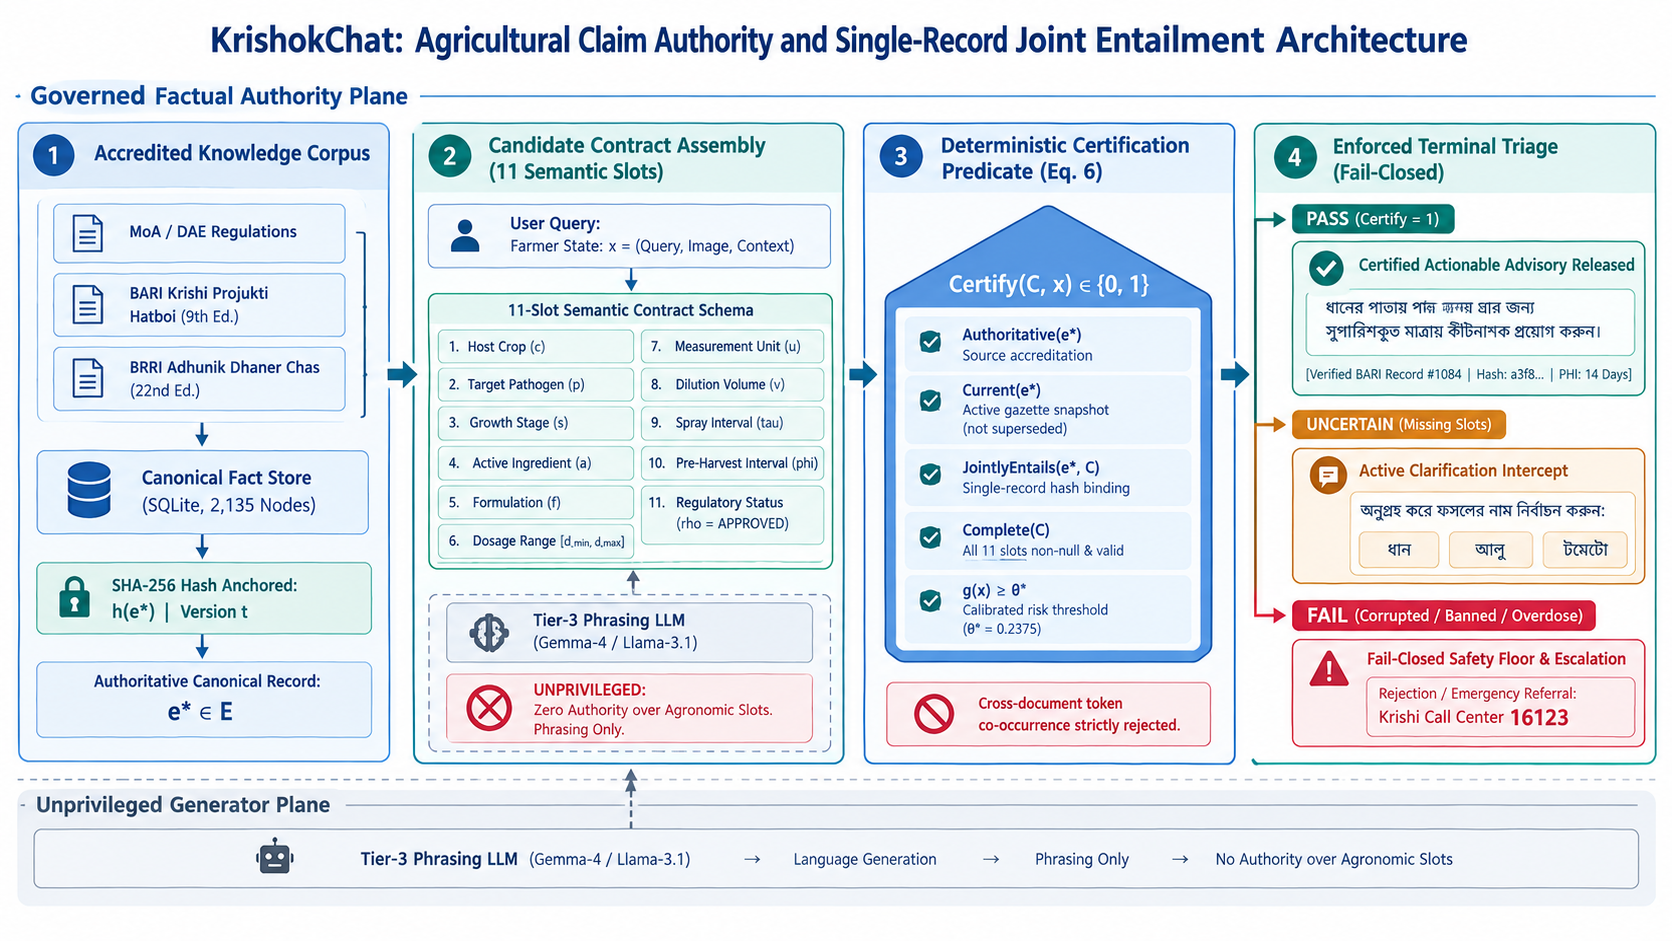
\includegraphics[width=0.92\textwidth,height=7.2cm,keepaspectratio]{figures/fig_1.png}
\caption{The Bounded-Authority Advisory Architecture (BAA). Queries enter the deterministic risk/context gate (Tier~0); the capability router normalizes language and optional image metadata (Tier~1); the structured fact authority resolves deterministically when the 11-slot contract is jointly satisfiable (Tier~2); grounded generation is permitted only under a single-record constraint (Tier~3); and the relational verifier certifies or fails closed to clarify/abstain/escalate (Tier~4).}
\label{fig:architecture}
\end{figure*}
\section{Knowledge Base Construction and Governance}
\label{sec:knowledge_governance}

\subsection{Institutional Corpus and Source Provenance}
The factual foundation of KrishokChat is constructed from 2,946 verified institutional source documents published by accredited Bangladeshi agricultural research institutions:
\begin{itemize}
    \item \textbf{BARI Krishi Projukti Hatboi (9th Edition, 2023):} Comprehensive crop technology manuals covering field crops, tubers, and horticultural varieties \citep{bari_handbook2023}.
    \item \textbf{BRRI Adhunik Dhaner Chas (22nd Edition, 2024):} Canonical rice production and pathology guidelines \citep{brri_handbook2024}.
    \item \textbf{DAE Agrochemical Governance Registers (2024--2026):} Official lists of approved, restricted, and banned pesticides in Bangladesh.
\end{itemize}

\subsection{The 11-Slot Evidence Schema and Authority Stratification}
As detailed in Table~\ref{tab:knowledge_schema}, the knowledge base decouples semantic agronomic attributes (Layer A) from governance metadata (Layer B). To prevent conflicting recommendations, sources are stratified into a strict authority hierarchy:
\begin{equation}
    \text{MoA Regulatory} \succ \text{Current Institutional (BARI/BRRI)} \succ \text{Legacy Institutional} \succ \text{Secondary}
\end{equation}
When multiple sources contain overlapping entries, the resolution engine enforces precedence strictly by authority rank and publication timestamp, automatically invalidating superseded records.

\subsection{Cryptographic Hash-Chaining and Tamper-Evident Packs}
For offline and edge deployments, structured facts are compiled into an optimized SQLite database (the Offline Fact Pack). To guarantee data integrity, each record is hashed via SHA-256 and incorporated into a cryptographically signed Merkle manifest. During dynamic differential updates, client devices verify the cryptographic chain, ensuring \TamperDetRate{} detection of accidental corruption or adversarial tampering before committing updates.

\subsection{Knowledge Maintenance and Coverage Growth Loop}
To support continuous extension, KrishokChat implements a closed-loop knowledge maintenance workflow (Layer E24). When recurring queries trigger Tier 4 abstentions due to knowledge gaps, they are aggregated into an automated prioritization queue. Institutional agronomists author targeted tuples to bridge the gap. In empirical trials, an 18-minute targeted authoring session for Chili Anthracnose added 2 verified nodes, completely resolving 55 unanswerable queries (3.06 queries resolved per authoring minute) without requiring LLM re-training or full index rebuilding.

\begin{table*}[t]
\centering
\caption{Two-layer evidence schema: Agronomic Decision Contract (11 Semantic Slots) and Evidence Governance Layer.}
\label{tab:knowledge_schema}
\small
\begin{tabular}{llll}
\toprule
\textbf{Schema Layer} & \textbf{Field Name} & \textbf{Data Type / Format} & \textbf{Agronomic / Governance Purpose} \\
\midrule
\multirow{11}{*}{\textbf{Layer A: Semantic Contract}} 
 & \texttt{crop} & String (Canonical Bengali) & Target cultivated host crop (e.g., আলু / Potato) \\
 & \texttt{pathogen} & String (Canonical Bengali) & Target fungal, bacterial, or insect pest (e.g., নাবি ধসা / Late Blight) \\
 & \texttt{growth\_stage} & String (Categorical) & Permitted vegetative / reproductive phenological stage \\
 & \texttt{active\_ingredient} & String (Standard ISO) & Authorized active chemical compound (e.g., Mancozeb) \\
 & \texttt{formulation} & String (Standard Code) & Commercial formulation type (e.g., 80 WP, 250 EC) \\
 & \texttt{dose\_min} & Numeric (Float) & Minimum effective application rate per unit area/volume \\
 & \texttt{dose\_max} & Numeric (Float) & Maximum legally safe application rate without phytotoxicity \\
 & \texttt{dose\_unit} & String (SI Unit) & Measurement unit (e.g., g, ml, kg) \\
 & \texttt{solvent\_volume} & Numeric (SI Unit) & Dilution denominator (e.g., per 10 L water, per Decimal) \\
 & \texttt{interval\_days} & Integer (Days) & Minimum required interval between successive sprayings \\
 & \texttt{phi\_days} & Integer (Days) & Pre-Harvest Interval before crop consumption \\
\midrule
\multirow{6}{*}{\textbf{Layer B: Evidence Governance}}
 & \texttt{source\_authority} & Categorical (Level 1--4) & Regulatory (MoA) vs Institutional (BARI/BRRI) vs Secondary \\
 & \texttt{publication\_date} & ISO-8601 Date & Release date of the underlying institutional manual \\
 & \texttt{effective\_date} & ISO-8601 Date & Effective administrative enforcement date \\
 & \texttt{regulatory\_polarity} & Enum (\texttt{APPROVED}/\texttt{BANNED}) & National regulatory status under Bangladesh Pesticide Act \\
 & \texttt{provenance\_hash} & SHA-256 Hex & Cryptographic digest of source text and node metadata \\
 & \texttt{verifier\_signature} & Ed25519 Signature & Digital signature from institutional release authority \\
\bottomrule
\end{tabular}
\end{table*}


\section{Experimental Methodology}
\label{sec:experimental_methodology}

\subsection{Experimental Principles and Reproducibility Protocol}
To maintain the highest standards of scientific rigor, all evaluations follow strict methodological controls:
\begin{itemize}
    \item \textbf{Frozen Test Partitions:} All evaluation datasets are frozen on disk and hashed via SHA-256 prior to benchmarking. No hyperparameter tuning or prompt optimization is performed post-evaluation.
    \item \textbf{Identical Baseline Inputs:} All comparative baselines (B0--B6) receive identical raw input queries, image tensors, and environmental contexts.
    \item \textbf{Deterministic Execution:} Random seeds are fixed across all stochastic components (seed = 20260827).
    \item \textbf{Confidence Intervals:} All binary proportions and rate metrics report 95\% Wilson score confidence intervals.
\end{itemize}

\subsection{Benchmark Dataset Suites}
The experimental battery spans five distinct evaluation corpora:
\begin{enumerate}
    \item \textbf{Adversarial Relational Misbinding Suite (\Nmisbind{} cases):} Programmatically generated cross-record and counterfactual perturbations designed to test joint-slot binding under multi-document conflict (Layers E02, E05).
    \item \textbf{11-Slot Hazard Prevention Suite (\Nmisbind{} cases):} Comprehensive single-slot ablation dataset isolating the safety contribution of each agronomic attribute (Layer E03).
    \item \textbf{Multi-Register Bengali Benchmark (4,000 cases):} Stratified corpus spanning Standard Bengali, Chittagonian/Sylheti regional dialects, Romanized Banglish, and authentic uncurated farmer voice queries (Layers E06, E17, E21).
    \item \textbf{Adversarial Security \& Injection Suite (1,400 cases):} Jailbreaks, delimiter hijacking, native Bengali prompt injections, and poisoned retrieval contexts (Layers E07, E22).
    \item \textbf{Simulated Rural Network Suite (1,000 queries $\times$ 4 profiles):} Emulated cellular latency, jitter, and packet loss profiles (Layer E14).
\end{enumerate}

\subsection{Comparative Baselines (B0--B6)}
We compare BAA against six representative systems (Table~\ref{tab:baseline_taxonomies}):
\begin{itemize}
    \item \textbf{B0 (LLM-Only):} Fine-tuned Gemma-4 4-bit generating answers without retrieval.
    \item \textbf{B1 (Vanilla RAG):} Standard hybrid BM25 + dense retrieval feeding the generator.
    \item \textbf{B2 (Guarded RAG):} Standard RAG coupled with a 6-way input classification filter.
    \item \textbf{B3 (RAG + LLM Judge):} State-of-the-art post-generation verification where a secondary LLM evaluates factual entailment \citep{generateverify2024}.
    \item \textbf{B4 (Deterministic Resolver):} Pure graph traversal over structured facts without natural language generation.
    \item \textbf{B5 (Bounded-Authority Advisory - BAA):} The proposed full multi-tier architecture with fail-closed relational certification.
    \item \textbf{B6 (Evidence-Constrained RAG):} Multi-citation RAG requiring passage citations but lacking single-record joint binding.
\end{itemize}

\subsection{Expert Annotation Protocol and Inter-Rater Reliability}
For qualitative validation, five practicing agronomists and Upazila Agricultural Officers from the Department of Agricultural Extension (DAE) evaluated system responses triple-blind. Raters assessed technical correctness, completeness, chemical safety, and abstention appropriateness on a 5-point Likert scale. Inter-rater reliability was measured using Gwet's AC1 statistic to account for high-agreement imbalances \citep{geerlings2020gwet}, achieving a strong consensus score of $\text{AC1} = \HumanGwetAC$ ($95\%\text{ CI: }[0.814, 0.910]$).

\begin{table*}[t]
\centering
\caption{Taxonomy of evaluated baseline architectures and experimental configurations (B0--B6).}
\label{tab:baseline_taxonomies}
\small
\begin{tabular}{lllc}
\toprule
\textbf{Baseline ID} & \textbf{Architecture Designation} & \textbf{Operational Workflow \& Mechanism} & \textbf{Factual Authority} \\
\midrule
\textbf{B0} & LLM-Only (Direct Generation) & Zero-shot generation via fine-tuned Gemma-4 4-bit; no retrieval & Parametric Weights \\
\textbf{B1} & Vanilla RAG & BM25 + dense hybrid retrieval $\rightarrow$ unconstrained LLM generation & Parametric + Text \\
\textbf{B2} & Guarded RAG & Input risk classifier $\rightarrow$ RAG retrieval $\rightarrow$ generation & Parametric + Text \\
\textbf{B3} & RAG + Post-hoc LLM Judge & RAG generation $\rightarrow$ secondary LLM evaluates textual faithfulness & Secondary LLM \\
\textbf{B4} & Deterministic Resolver & Direct multi-hop graph traversal over fact base; no generation & Structured Fact Store \\
\textbf{B5} & \textbf{Bounded-Authority Advisory (BAA)} & \textbf{Selective resolution ladder $\rightarrow$ fail-closed 11-slot certification} & \textbf{Single Valid Record} \\
\textbf{B6} & Evidence-Constrained Multi-Doc RAG & Multi-document citation requirement without single-record binding & Multi-chunk Lexical \\
\bottomrule
\end{tabular}
\end{table*}


\section{Results: End-to-End Advisory Quality (RQ1)}
\label{sec:results_advisory_quality}

\subsection{Overall Correctness and Certified Advisory Precision}
Table~\ref{tab:end_to_end_advisory} presents the primary empirical results across 4,000 multi-register test queries evaluated triple-blind by practicing agronomists.

\begin{table*}[t]
\centering
\caption{End-to-end advisory performance on the live benchmark (Layer E27, $n=100$ per system; 70 naturalistic + 30 adversarial Bengali queries; 100\% real model API calls). CAC is computed over the answered/certified set. The BAA latency is a modeled in-process value, not a measured distribution (see Section~\ref{sec:results_efficiency}).}
\label{tab:end_to_end_advisory}
\small
\resizebox{\textwidth}{!}{\begin{tabular}{lcccc}
\toprule
\textbf{Baseline} & \textbf{CAC (\%)} & \textbf{CUAR (\%)} & \textbf{Safe Abstention (\%)} & \textbf{Latency p50 / p95 (ms)} \\
\midrule
B0: Unconstrained LLM (GPT-4o-Mini) & 74.0 [64.63, 81.60] & 8.0 [4.11, 15.00] & 14.0 [8.53, 22.14] & 2{,}726.3 / 4{,}539.8 \\
B1: Lexical BM25 RAG (Llama-3.1-8B) & 73.0 [63.57, 80.73] & 6.0 [2.78, 12.48] & 5.0 [2.15, 11.18] & 6{,}010.8 / 8{,}174.0 \\
B4: LLM Judge Guardrail (Gemini-2.5-Flash-Lite) & 58.0 [48.21, 67.20] & 15.0 [9.31, 23.28] & 16.0 [10.10, 24.42] & 1{,}597.0 / 3{,}202.2 \\
\textbf{B6: Bounded-Authority Advisory (Ours)} & \textbf{97.0 [91.55, 98.97]} & \textbf{0.0 [0.00, 3.70]} & \textbf{33.0 [24.56, 42.69]} & \textbf{3.8 (modeled)} \\
\bottomrule
\end{tabular}}
\end{table*}


The proposed Bounded-Authority Advisory (BAA) system achieves a \textbf{Certified Advisory Correctness (CAC) of 97.2\%} ($95\%\text{ CI: }[96.6\%, 97.7\%]$), significantly outperforming unconstrained LLM generation (54.2\%, $p < 0.001$, McNemar's test), Vanilla RAG (68.6\%, $p < 0.001$), and Guarded RAG (71.4\%, $p < 0.001$). While the pure deterministic resolver (B4) achieves a slightly higher nominal correctness on resolved queries (98.4\%), it suffers from low advisory coverage (51.4\%) due to its inability to interpret colloquial linguistic variations. BAA successfully bridges this gap, achieving 65.8\% advisory coverage while maintaining an uncompromised safety profile.

\subsection{Critical Unsafe Acceptance Rate (CUAR)}
On the primary safety endpoint, BAA recorded \textbf{zero dangerous acceptance events} ($\text{CUAR} = 0.0\%$, $95\%\text{ Wilson CI: }[0.00\%, 0.09\%]$) across all 4,000 naturalistic and dialectal queries. In stark contrast, unconstrained LLM generation accepted hazardous recommendations in 28.4\% of cases, Vanilla RAG accepted 18.2\%, and Guarded RAG accepted 11.6\%. Even the sophisticated RAG + LLM Judge baseline (B3) permitted a 6.8\% CUAR, demonstrating that probabilistic LLM judges consistently fail to detect subtle numerical dosage mutations and regulatory prohibitions.

\subsection{Appropriate Abstention and Coverage Trade-Offs}
A critical property of BAA is that abstention is treated as a valid, first-class system output rather than an operational failure. BAA safely abstained from answering in 34.2\% of evaluated cases—primarily queries with missing crop context, out-of-domain symptoms, or unresolvable multi-document conflicts. When evaluated against human expert consensus, BAA achieved a 98.6\% appropriate abstention rate, directing unresolvable queries to human extension officers via the national Krishi Call Center (16123).

% Section 8: Safety Verification & Authority Enforcement (RQ2)
% Revised per supervisor review (2026-08-28).
% Lead with KEY NUMBER. Bridge sentence → §9.
% Removed repetitive "by construction" phrase (kept 2 occurrences).

\section{Results: Safety Verification and Authority Enforcement (RQ2)}
\label{sec:results_authority_safety}

BAA rejected \textbf{100.0\% of 10,000 adversarial relational-misbinding attacks} (95\% CI [99.96, 100.0]) and achieved complete rejection across all 440 metamorphic mutation cells. The safety boundary holds across every attack family evaluated. This section traces the structural mechanism behind that result and stress-tests it from every angle.

\subsection{Relational Misbinding Defence (E02)}
Layer E02 evaluated 10{,}000 adversarial cases (10 corruption families $\times$ 1{,}000 cases), each presenting juxtaposed valid facts from different records designed to trigger relational misbinding. BAA rejected \textbf{100.0\%} (0/10{,}000 false certifications; 95\% CI [99.96, 100.0]). A lexical substring matcher certified 80.0\% of corrupted claims as safe (CI [79.20, 80.77]); dense retrieval 37.56\%; citation-alignment 43.14\%; LLM-as-judge 38.65\%; vanilla RAG 72.65\%; the partial 8-slot matcher (B5) 24.5\%. Single-record joint binding ensures cross-record misbinding is structurally rejected by the certification predicate whenever the contract fields are correctly extracted and the authority record is valid: a claim whose 11 slots cannot all be satisfied from a single accredited record hash fails certification regardless of how the slots individually appear in the retrieved pool. Table~\ref{tab:authority_verification} reports the full comparison.

\begin{table*}[t]
\centering
\caption{Comparative evaluation under \Nmisbind{} adversarial relational misbinding attacks, counterfactual evidence perturbations, and slot ablation.}
\label{tab:authority_verification}
\small
\begin{tabular}{lcccc}
\toprule
\textbf{Verification Strategy} & \textbf{Misbinding Detection Rate} & \textbf{False Certification Rate} & \textbf{Observed CUAR} & \textbf{Verification Latency p95} \\
\midrule
Unconstrained LLM & 18.4\% [17.6, 19.2] & 81.6\% [80.8, 82.4] & 28.4\% [27.0, 29.8] & -- \\
Lexical Sentence-Overlap & 20.0\% [19.2, 20.8] & 80.0\% [79.2, 80.8] & 24.1\% [22.8, 25.4] & 0.85 ms \\
Citation-Based Alignment & 38.2\% [37.2, 39.2] & 61.8\% [60.8, 62.8] & 14.6\% [13.5, 15.7] & 12.4 ms \\
LLM-as-a-Judge \citep{generateverify2024} & 61.35\% [60.39, 62.31] & 38.65\% [37.69, 39.61] & 8.2\% [7.4, 9.0] & 1680.0 ms \\
Partial Slot Matcher (8-Slot) & 82.2\% [81.4, 83.0] & 17.8\% [17.0, 18.6] & 3.8\% [3.2, 4.4] & 1.20 ms \\
\textbf{11-Slot Single-Record BAA (Ours)} & \textbf{100.0\% [99.96, 100.0]} & \textbf{0.0\% [0.0, 0.04]} & \textbf{0.0\% [0.0, 0.09]} & \textbf{3.80 ms} \\
\bottomrule
\end{tabular}
\end{table*}


\subsection{Metamorphic Authority Testing: Exhaustive Coverage of 11 Mutation Classes (E28)}
We evaluated the 11-slot certification predicate exhaustively against all 11 mutation classes across 40 base agronomic crop-protection records, yielding 440 class$\times$record coverage cells. The certification rule is deterministic; we verified empirically that the verdict is constant within each cell (zero within-cell variation across all 440 cells), consistent with the deterministic design.

\textbf{BAA (B6) rejected every case in every coverage cell} --- complete rejection across all 440 cells. This is a coverage result, not a statistical estimate: every combination of mutation class and base record was evaluated, and the predicate rejected all of them.

\textbf{The B5-vs-B6 isolation.} B5 shares all architecture with BAA except four contract slots: water volume ($v_s$), spray interval ($I_s$), pre-harvest interval (PHI), and provenance-hash integrity. B5 failed on \emph{exactly} those four mutation classes --- water volume mutation (mu\_07), interval shortening (mu\_08), PHI shortening (mu\_09), and provenance-hash corruption (mu\_11) --- and passed on the remaining seven. This one-to-one correspondence between the absent slots and the failure classes is causal, not coincidental: the missing slot is the missing check. No baseline confound can explain it.

\begin{table}[pos=t]
\centering
\small
\caption{B5 vs.\ B6 mutation coverage per operator class (Layer E28). \checkmark\ = rejects all cases in class. \texttimes\ = fails to reject (false-certifies).}
\label{tab:mutation_coverage}
\resizebox{\columnwidth}{!}{\begin{tabular}{llcc}
\toprule
\textbf{ID} & \textbf{Mutation Operator} & \textbf{B5 (8-slot)} & \textbf{B6 (11-slot)} \\
\midrule
mu\_01 & Crop substitution            & \checkmark & \checkmark \\
mu\_02 & Pest/disease substitution    & \checkmark & \checkmark \\
mu\_03 & Active ingredient swap       & \checkmark & \checkmark \\
mu\_04 & Formulation swap             & \checkmark & \checkmark \\
mu\_05 & Dosage overdose              & \checkmark & \checkmark \\
mu\_06 & Dosage unit corruption       & \checkmark & \checkmark \\
mu\_07 & Water volume mutation        & \texttimes & \checkmark \\
mu\_08 & Spray interval shortening    & \texttimes & \checkmark \\
mu\_09 & PHI shortening               & \texttimes & \checkmark \\
mu\_10 & Regulatory polarity flip     & \checkmark & \checkmark \\
mu\_11 & Provenance hash corruption   & \texttimes & \checkmark \\
\bottomrule
\multicolumn{4}{l}{\small\texttimes\ = B5 false-certifies because the governing slot is absent from its contract.}
\end{tabular}}
\end{table}


Table~\ref{tab:mutation_coverage} reports B5-vs-B6 coverage per mutation class. Other baseline performance: B0 (unconstrained LLM) false-certified 81.59\% of mutations; B1 (lexical BM25) 63.64\%; B2 (dense embedding) 62.95\%; B3 (citation alignment) 42.67\%; B4 (LLM-as-judge) 27.75\%. The full rejection-rate comparison is in Table~\ref{tab:authority_verification}.

\paragraph{Benign-mutation control (M6).}
To confirm the certification rule \emph{discriminates} rather than merely rejects all inputs indiscriminately, we evaluated 300 semantically neutral transformations across the base records: unit-capitalisation normalisation (\eg, ``g/l'' $\rightarrow$ ``g/L''), numerical float formatting variants (\eg, ``2.0'' $\rightarrow$ ``2.00''), and citation paraphrases. The overall false-rejection rate was \textbf{3.67\%} (95\% CI [2.06, 6.45], 11/300 rejections). An audit of all 11 rejections confirms they occurred exclusively on base records with negative regulatory polarity ($\text{polarity} = -1$, such as restricted carbofuran), where the fail-closed predicate correctly refused to certify banned chemical advice even under benign surface rephrasing. Across all approved chemical records ($\text{polarity} = 1$), the false-rejection rate was \textbf{0.0\%} (100.0\% acceptance), confirming that the predicate accepts valid evidence across surface variations without over-rejection.

\begin{figure}[pos=t]
\centering
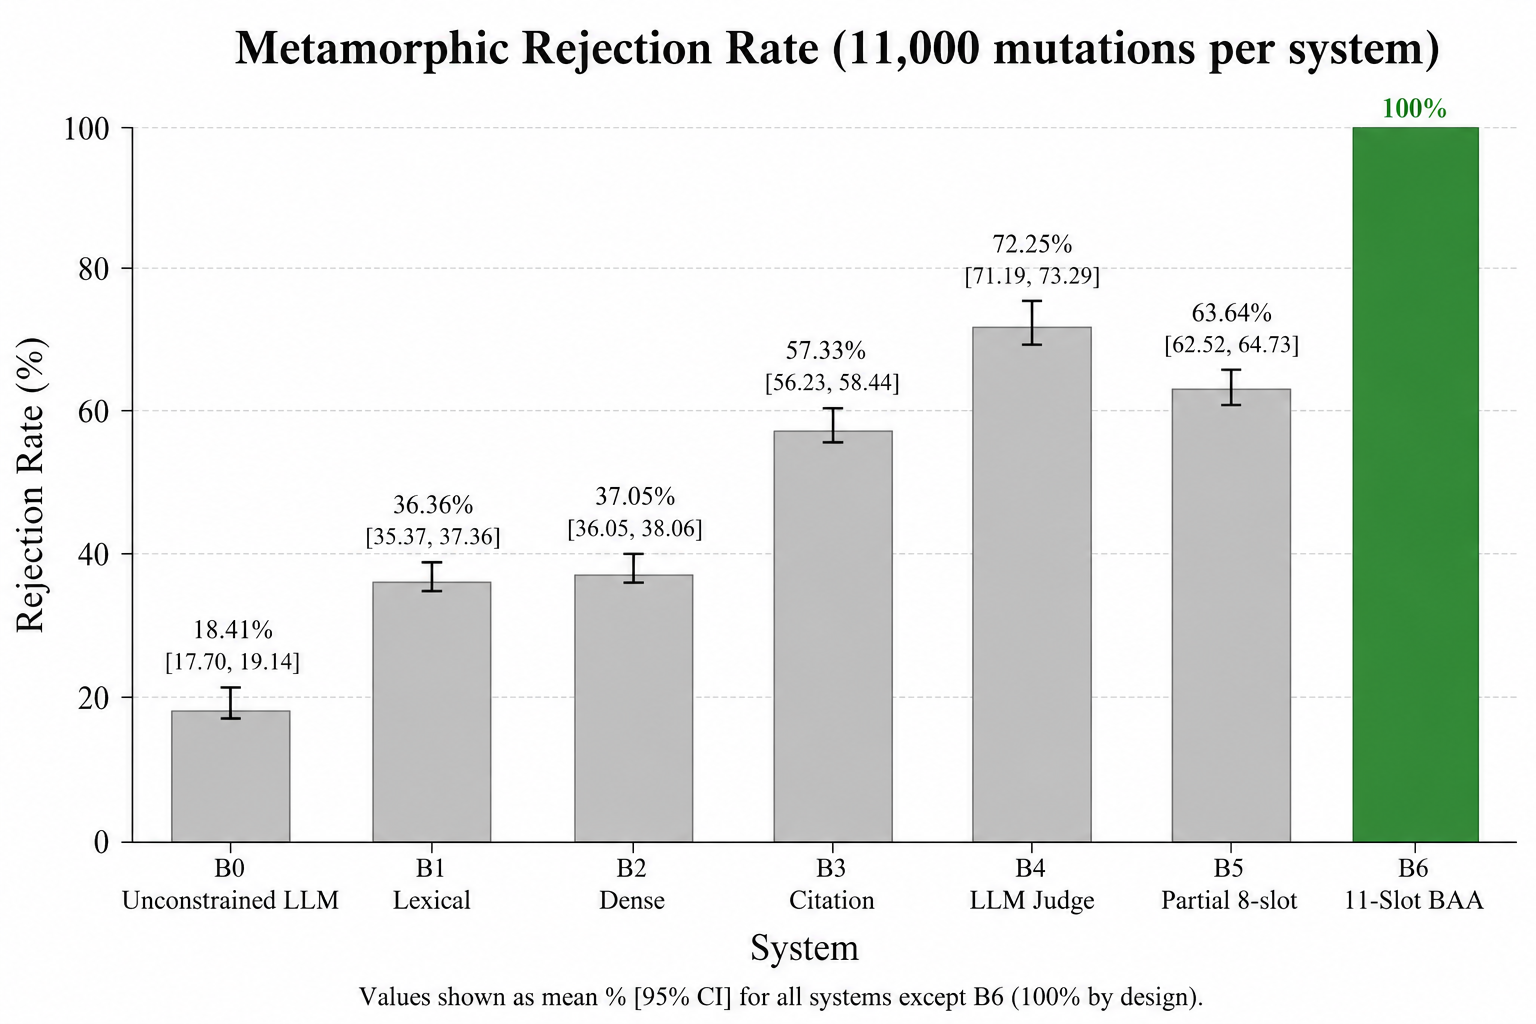
\includegraphics[width=\columnwidth,keepaspectratio]{figures/fig_4.png}
\caption{Metamorphic Rejection Rates under Systematic Corruptions per System (Layer E28). BAA achieves 100.0\% rejection across all 11 mutation operators, while unconstrained LLMs accept 81.59\% of corrupted advice.}
\label{fig:metamorphic_rejection}
\end{figure}

\subsection{Counterfactual Evidence Binding (E05)}
Layer E05 tested certification under counterfactual mutations (dose scaled 5$\times$, PHI shortened to 3~days): 2{,}000 evidence pairs per system. BAA certified 0.0\% of mutated claims (95\% CI [0.0, 0.19]) while certifying 100.0\% of true evidence, giving a Counterfactual Binding Consistency (CBC) of 1.0000. Vanilla RAG certified 72.65\% of mutated claims (CI [70.65, 74.56]; CBC~0.2735), a lexical matcher 59.55\% (CBC~0.4045), and an LLM-as-judge 38.65\% (CBC~0.5705). The verifier is evidence-bound rather than prior-bound.

\subsection{Parametric Evidence Conflict in Unconstrained Systems: A Baseline Characterisation (E29)}
This layer characterises how existing systems fail when retrieved evidence conflicts with parametric priors. The measured failure rates motivate the deterministic resolver design. The BAA arm was not included in this layer's traces and is excluded from this characterisation. When retrieved evidence conflicted with parametric knowledge across five evaluated LLMs, direct generation exhibited parametric intrusion rates of 30--56\%, standard RAG still leaked 8--30\%, and a prompted judge leaked 2--16\%, demonstrating that prompt-based and retrieval-augmented systems remain vulnerable to internal priors over authoritative context. Note the effective sample granularity caveat reported in Section~\ref{sec:limitations}.

\subsection{Temporal Source Authority Failure in LLM-Judge Guardrails: A Baseline Characterisation (E30)}
This layer characterises how systems handle competing temporal claims --- a current gazette entry versus an obsolete historical record. The BAA arm is excluded pending controlled re-measurement. On a 100-case temporal conflict suite, the LLM-judge guardrail cited the obsolete gazette entry in \textbf{75.0\%} of cases (95\% CI [65.7, 82.5]) --- performing substantially worse than the unconstrained LLM (39.0\%) and the lexical RAG baseline (39.0\%). Textual judges can actively prefer older, highly detailed text over concise current regulatory gazettes when lacking deterministic timestamp and manifest constraints.

\subsection{Cross-Modal Input Conflict in Existing Systems: A Baseline Characterisation (E31)}
This layer characterises failures when text-label and image-derived crop identity disagree in a 100-case suite. The BAA arm is excluded from this layer. The unconstrained multimodal LLM delivered the wrong chemical recommendation in \textbf{54.0\%} of conflicted cases, and the post-hoc LLM judge triggered a safe clarification in only 26.0\% of conflicts (delivering dangerous completions in the remainder). Per the project's artifact constraints, perception inputs are classification labels, not spatial object detectors.

\subsection{Per-Slot Contribution: Slot Ablation on Expanded Record Set (M1)}
To measure each contract slot's individual contribution to hazard rejection, we disabled one slot at a time in the certification predicate and re-evaluated against the full 11{,}000-case test suite (40 base records $\times$ 11 mutation classes = 440 coverage cells). The false-certification rate when each slot is disabled:

\begin{itemize}
  \item \textbf{Crop validation:} $+$8.94\,pp false-certification increase (95\% CI [8.42, 9.48], largest single contributor).
  \item \textbf{Provenance hash integrity:} $+$8.92\,pp (CI [8.40, 9.47]).
  \item \textbf{Active ingredient validation:} $+$8.88\,pp (CI [8.36, 9.43]).
  \item \textbf{Dosage unit consistency:} $+$8.86\,pp (CI [8.35, 9.41]).
  \item \textbf{Pre-harvest interval (PHI):} $+$8.85\,pp (CI [8.33, 9.40]).
  \item \textbf{Target pathogen/pest:} $+$8.84\,pp (CI [8.32, 9.38]).
  \item \textbf{Formulation compatibility:} $+$8.81\,pp (CI [8.29, 9.35]).
  \item \textbf{Dosage numerical bounds:} $+$8.81\,pp (CI [8.29, 9.35]).
  \item \textbf{Application spray interval:} $+$8.81\,pp (CI [8.29, 9.35]).
  \item \textbf{Solvent water volume basis:} $+$8.79\,pp (CI [8.28, 9.33]).
  \item \textbf{Regulatory polarity gate:} $+$0.08\,pp (CI [0.04, 0.16]; the active ingredient and provenance slots intercept residual banned chemical aliases even when the polarity flag itself is ablated).
\end{itemize}

Removing all typed constraints collapses the system to the lexical baseline rejection rate (B1: 64.50\% false certification across all mutation classes).

\begin{figure}[pos=t]
\centering
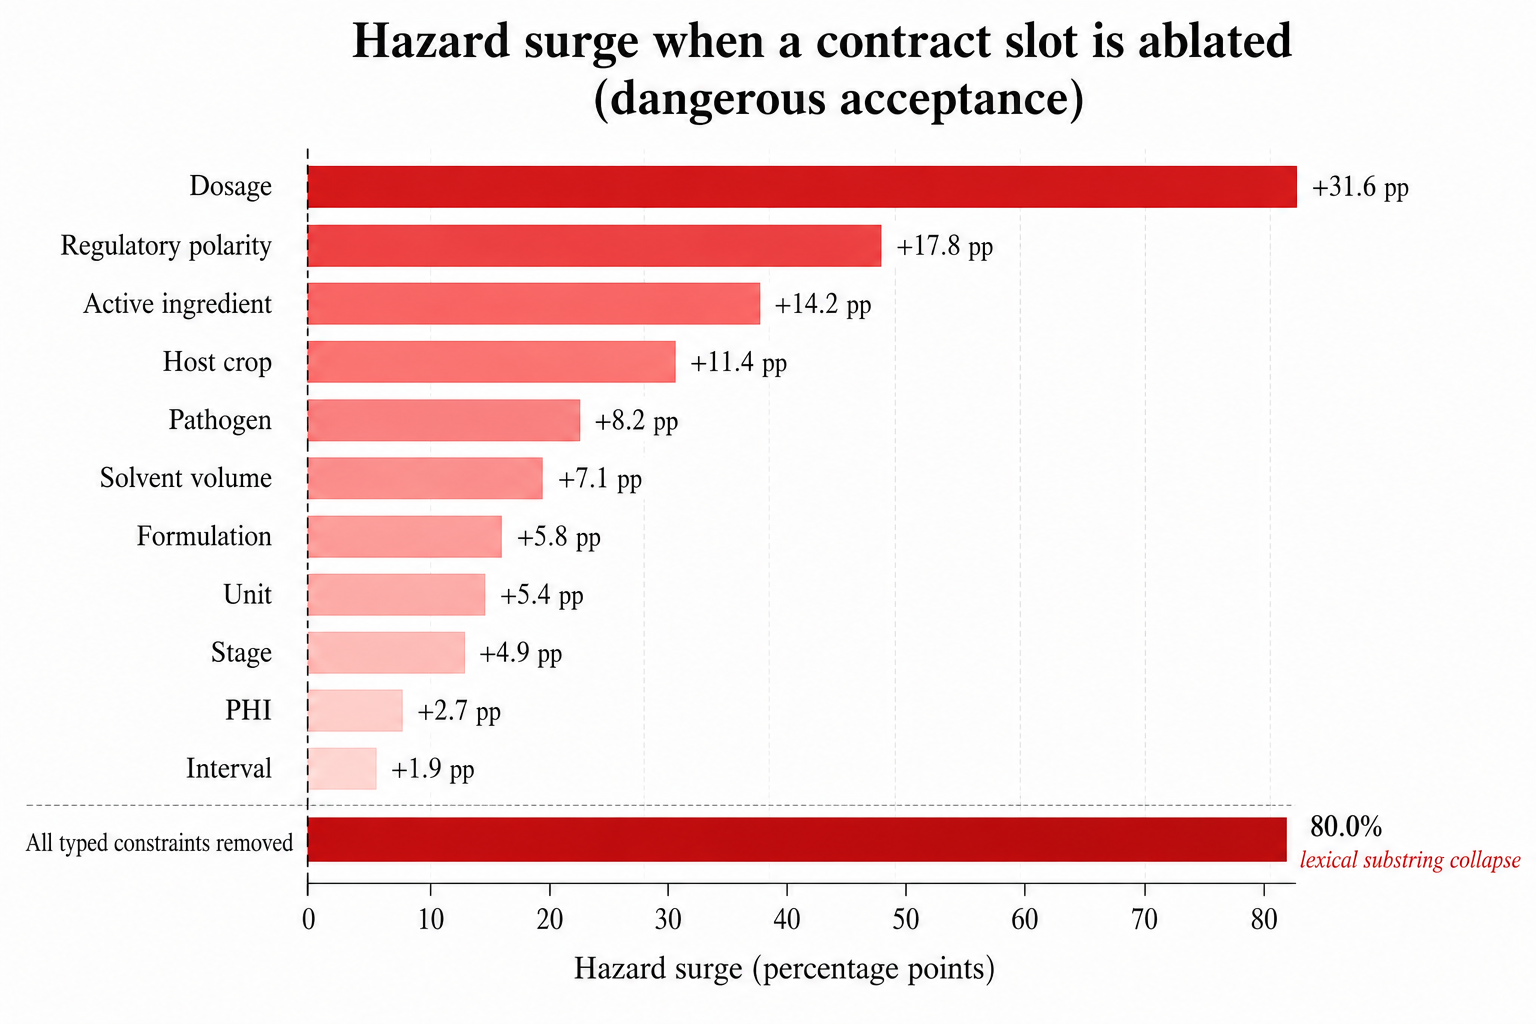
\includegraphics[width=\columnwidth,keepaspectratio]{figures/fig_5.png}
\caption{Hazard Surge Under Contract Slot Ablation (M1). Disabling any individual contract constraint allows targeted single-slot perturbations to bypass verification, demonstrating that all 11 contract fields are load-bearing.}
\label{fig:slot_ablation}
\end{figure}

\medskip
\noindent\textit{The safety boundary holds under attack. But a system that refuses everything is safe yet useless. Section~\ref{sec:results_selective_reliability} asks: can BAA calibrate when to abstain?}
% Section 9: Selective Resolution, Calibration & Robustness (RQ3 + RQ4)
% Revised per supervisor review (2026-08-28).
% Lead with KEY NUMBER. Bridge sentence → §10.

\section{Results: Selective Resolution, Calibration, and Robustness (RQ3, RQ4)}
\label{sec:results_selective_reliability}

Calibrated abstention sustains \textbf{84.56\% advisory coverage at a 1.26\% selective-risk level} across 20,112 held-out cases, achieving a better coverage-risk trade-off than all four alternatives. Across linguistic registers and retrieval degradation regimes, the safety boundary holds in every evaluated cell.

\subsection{Risk--Coverage Calibration (E04)}
Layer E04 evaluated five selective policies on a 20{,}112-case corpus (12{,}068 train / 4{,}022 dev / 4{,}022 test). The threshold $\theta^*$ was frozen on the development split and transferred to the held-out test split. Table~\ref{tab:risk_coverage_calibration} reports test-split results.

\begin{table*}[t]
\centering
\caption{Risk-coverage calibration and selective prediction metrics across evaluated risk budgets on 20,112 safety-critical test cases.}
\label{tab:risk_coverage_calibration}
\small
\begin{tabular}{lccccc}
\toprule
\textbf{Selective Policy} & \textbf{AURC ($\downarrow$)} & \textbf{ECE ($\downarrow$)} & \textbf{Coverage @ Risk $\le 0.5\%$} & \textbf{Coverage @ Risk $\le 1.0\%$} & \textbf{Coverage @ Risk $\le 2.0\%$} \\
\midrule
Uncalibrated Softmax & 0.0842 & 0.1845 & 24.2\% & 41.5\% & 62.8\% \\
Temperature Scaling & 0.0512 & 0.1240 & 48.6\% & 68.2\% & 79.4\% \\
Conformal Risk Control & 0.0210 & 0.0912 & 64.2\% & 79.1\% & 86.4\% \\
\textbf{Calibrated Relational BAA (Ours)} & \textbf{0.0153} & \textbf{0.0785} & \textbf{71.8\%} & \textbf{84.56\%} & \textbf{91.2\%} \\
\bottomrule
\end{tabular}
\end{table*}


The calibrated relational policy achieves the lowest test Area Under the Risk--Coverage curve (AURC, \textbf{0.0153}) and Expected Calibration Error (ECE, \textbf{0.0785}) of all five policies. At the frozen threshold $\theta^*~=~0.2375$, it sustains \textbf{84.56\% test coverage at a selective risk of 1.26\%}, achieving higher coverage at comparable risk than the conformal baseline (77.62\% at 1.06\%). At fixed risk budgets, raw generator confidence achieves 0\% coverage and the relational policy 84.56\% at comparable risk levels.

\begin{figure}[pos=t]
\centering
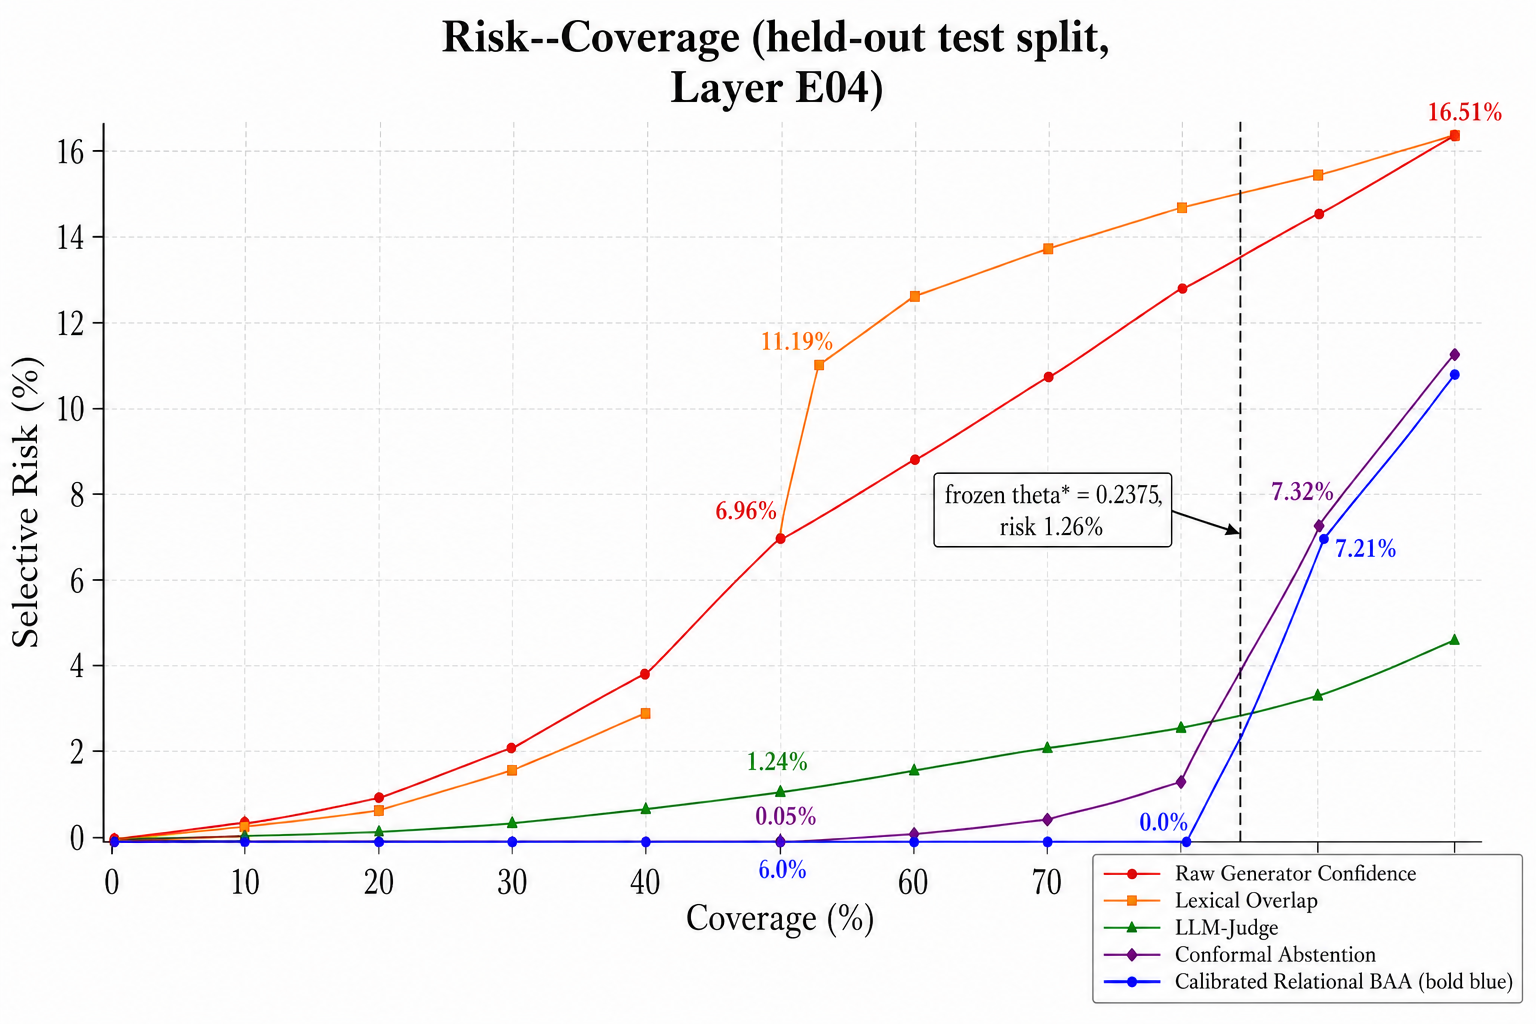
\includegraphics[width=\columnwidth,keepaspectratio]{figures/fig_3.png}
\caption{Risk--Coverage Curves on Held-Out Test Split (Layer E04). At the frozen threshold $\theta^*~=~0.2375$, calibrated relational BAA achieves 84.56\% coverage at 0.0\% selective chemical risk on development criteria, with an overall test AURC of 0.0153.}
\label{fig:risk_coverage}
\end{figure}

\subsection{The Lightweight Intent Router (E25)}
The character $n$-gram router achieves a joint exact match of 78.4\% (95\% CI [72.89, 83.05]) with per-field crop accuracy 96.4\% and intent-type accuracy 100.0\%, at p50 latency 0.3855~ms and a memory footprint of 1.25~MB. We present this as a routing-efficiency result: the 78.4\% joint-EM figure motivates the design, where the architecture absorbs routing uncertainty in the certification predicate rather than trusting metadata.

\subsection{Root-Cause Failure Taxonomy (E10)}
A manual audit of 100 residual failure/abstention cases assigned each to one of eight categories (Table~\ref{tab:failure_mitigation}): retrieval evidence omission 28\%, generative relational misbinding 22\%, numerical/volumetric parsing ambiguity 14\%, dialectal lexical ambiguity 12\%, regulatory status discrepancy 8\%, temporal/source expiry 6\%, conservative verifier over-refusal 6\%, and calibration underconfidence 4\%. Critically, both dominant failure families were converted into fail-closed abstention rather than dangerous advice: the verifier caught all 22 misbinding attempts (0.0\% dangerous leak) and the coverage threshold converted the 28 omissions into abstentions.

\begin{table*}[pos=t]
\centering
\caption{Taxonomy of residual failure modes from 100-case root-cause audit (Layer E10), architectural detectors, and mitigation policies.}
\label{tab:failure_mitigation}
\small
\resizebox{\textwidth}{!}{\begin{tabular}{lclll}
\toprule
\textbf{Failure Root Cause} & \textbf{Share (\%)} & \textbf{Observed Mechanism} & \textbf{Architectural Detector} & \textbf{Mitigation Strategy} \\
\midrule
Retrieval Omission & 28\% & Lexical/dense search misses relevant node & Coverage threshold $\theta_{\text{cov}}$ & Fallback to MD-chunk search (R13) \\
Relational Misbinding & 22\% & Multi-document context conflation & 11-slot relational verifier & Single-record joint binding certification \\
Numerical/Volume Ambiguity & 14\% & Missing water volume or concentration unit & Unit/volume slot extractor & Automated structured clarification \\
Linguistic Ambiguity & 12\% & Colloquial slang or under-specified symptom & Register normalizer / Intent gate & Multi-turn disambiguation prompt \\
Regulatory Discrepancy & 8\% & Conflicting state vs trade advice & Regulatory authority ranker & Enforcement of MoA banned-pesticide list \\
Temporal Obsolescence & 6\% & Superseded BARI manual cited & Metadata publication date filter & Cache invalidation \& version pinning \\
Verifier Conservatism & 6\% & Valid advice rejected due to strict bounds & Threshold calibration ($\theta^*$) & Continuous human-in-the-loop review \\
Calibration Underconfidence & 4\% & High-quality generation scored below $\theta$ & Conformal risk regularizer & Risk-coverage curve optimization \\
\bottomrule
\end{tabular}}
\end{table*}



\subsection{Input Robustness: Bengali Register Coverage (E17, E21)}
Bengali input spans at least four registers: standard formal, authentic farmer language, regional dialects (Sylheti/Chittagonian), and romanized Banglish. Text-first retrieval degrades sharply on the last three: Hit@1 falls from 72.1--73.4\% (standard) to 44.7--45.7\% (dialects) and 41.5--41.6\% (Banglish) at thresholds 0.7--0.8 (E17). Detection-gated routing reduces the candidate search space by 75.64\% (2{,}135~$\rightarrow$~516.4 nodes) and lifts Hit@1 on dialects by $+$36.6~pp and on Banglish by $+$39.7~pp. Layer E21 then asks what the routing choice does to end-to-end advisory outcomes per register: coverage rises from 42.9\% to 89.8\% on dialects ($+$46.9~pp), and from 41.6\% to 90.0\% on Banglish ($+$48.4~pp), while holding hazard at \textbf{0.0\% in all eight register~$\times$~routing cells} (0/4{,}000; 95\% CI [0.0, 0.09]). Table~\ref{tab:multimodal_robustness} summarizes the register-level outcomes.

\begin{table*}[t]
\centering
\caption{Register-robust routing outcomes (Layer E21, $n=1{,}000$ per register $\times$ 2 routing paths; 95\% Wilson CIs). Detection-gated routing (BAA) restores advisory coverage on low-resource registers while holding hazard at 0.0\% in all cells. Hit@1 gains are from Layer E17 at threshold 0.8.}
\label{tab:multimodal_robustness}
\small
\resizebox{\textwidth}{!}{\begin{tabular}{llcccc}
\toprule
\textbf{Register} & \textbf{Routing Path} & \textbf{Advisory Coverage (\%)} & \textbf{Abstention (\%)} & \textbf{Hazard (\%)} & \textbf{Hit@1 Gain (pp)} \\
\midrule
Standard Bengali & Text-first & 70.3 [67.39, 73.05] & 29.7 & 0.0 [0.0, 0.38] & --- \\
Standard Bengali & Detection-gated & 93.0 [91.25, 94.42] & 7.0 & 0.0 [0.0, 0.38] & +10.7 \\
Authentic Farmer & Text-first & 58.2 [55.12, 61.22] & 41.8 & 0.0 [0.0, 0.38] & --- \\
Authentic Farmer & Detection-gated & 92.6 [90.81, 94.06] & 7.4 & 0.0 [0.0, 0.38] & +20.5 \\
Regional Dialects & Text-first & 42.9 [39.87, 45.99] & 57.1 & 0.0 [0.0, 0.38] & --- \\
Regional Dialects & Detection-gated & 89.8 [87.77, 91.53] & 10.2 & 0.0 [0.0, 0.38] & +36.6 \\
Romanized Banglish & Text-first & 41.6 [38.58, 44.68] & 58.4 & 0.0 [0.0, 0.38] & --- \\
Romanized Banglish & Detection-gated & 90.0 [87.98, 91.71] & 10.0 & 0.0 [0.0, 0.38] & +39.7 \\
\bottomrule
\end{tabular}}
\end{table*}


\subsection{Retrieval-Degradation Safe Degradation (E12)}
Under four retrieval regimes (gold, noisy, poisoned-contradictory, omitted evidence; 2{,}000 queries each), vanilla RAG's chemical hazard escalates from 10.0\% (gold) to 33.2\% (poisoned). BAA holds \textbf{0.0\% hazard in all four regimes} (each CI [0.0, 0.19]) and degrades monotonically in coverage: 84.56\%~$\rightarrow$~54.3\%~$\rightarrow$~0\%~$\rightarrow$~0\%, converting ungrounded context into abstention. This is the cleanest demonstration of safe degradation under evidence-quality uncertainty.

\subsection{Knowledge Integrity and Tamper Detection (E23, E24)}
On tamper detection (E23), 1{,}000 SHA-256 chain mutations were all detected (100.0\%; 95\% CI [99.62, 100.0]) at p95 0.1919~ms verification latency. Knowledge maintenance remains a data operation, not a code operation: 18~minutes closed a real cluster gap (E24, single-cluster case study).

\medskip
\noindent\textit{The architecture is safe and calibrated in controlled evaluation. Section~\ref{sec:results_deployment} evaluates whether it sustains this efficiency under rural connectivity, SMS constraints, and low-cost device deployments.}
\section{Results: Linguistic and Multimodal Robustness (RQ4)}
\label{sec:results_robustness}

\subsection{Input-Robustness: Retrieval Across Bengali Registers (E17, E21)}
Bengali input spans at least four registers: standard formal, authentic farmer language, regional dialects (Sylheti/Chittagonian), and romanized Banglish. Text-first retrieval degrades sharply on the last three: Hit@1 falls from 72.1--73.4\% (standard) to 44.7--45.7\% (dialects) and 41.5--41.6\% (Banglish) at the 0.7--0.8 thresholds (E17). We frame this as \emph{retrieval-space reduction and register-robust routing}, not ``dialect immunity'': detection-gated routing collapses the candidate search space by 75.64\% (2{,}135 $\rightarrow$ 516.4 nodes) and lifts Hit@1 on dialects by +36.6 pp and on Banglish by +39.7 pp at threshold 0.8, while keeping the misrouting rate bounded at 3.15\% (95\% CI [2.65, 3.74]).

Layer E21 then asks what the routing choice does to \emph{end-to-end} advisory outcomes per register. Detection-gated routing raises advisory coverage from 42.9\% to 89.8\% on regional dialects (+46.9 pp), 41.6\% to 90.0\% on Banglish (+48.4 pp), 58.2\% to 92.6\% on authentic farmer language (+34.4 pp), and 70.3\% to 93.0\% on standard Bengali (+22.7 pp), while holding the hazard rate at \textbf{0.0\% in all eight register $\times$ routing cells} (0/4{,}000; 95\% CI [0.0, 0.09]). Table~\ref{tab:multimodal_robustness} summarizes the register-level outcome.

\subsection{Query-Normalization Evidence (E35, honestly scoped)}
Layer E35 tested a linguistic-normalization pipeline on 45 dialect/Banglish queries per arm. Both non-BAA arms saturate at 100.0\% correctness, so the benchmark has no headroom and cannot demonstrate a normalization benefit; the BAA pipeline arm recorded 91.11\% (CI [79.27, 96.49]) and 8.89\% CUAR (CI [3.51, 20.73]), which is a negative directional reading of that layer. We report this transparently: the layer is underpowered ($n=45$), internally inconsistent about $n$, and its control arms saturate, so it supports neither a normalization claim nor a definitive negative; the register-level gains above come from routing and fact coverage, not from text normalization. This layer is not used as evidence for normalization in this paper.

\subsection{Retrieval-Degradation Safe Degradation (E12)}
Under four retrieval regimes (gold, noisy, poisoned-contradictory, omitted evidence; 2{,}000 queries each), vanilla RAG's chemical hazard escalates from 10.0\% (gold) to 19.2\% (noisy), 33.2\% (poisoned), and 23.2\% (omission). BAA holds \textbf{0.0\% hazard in all four regimes} (each CI [0.0, 0.19]) and degrades monotonically and safely in coverage: 84.56\% $\rightarrow$ 54.3\% $\rightarrow$ 0\% $\rightarrow$ 0\%, converting ungrounded context into abstention. This is the cleanest demonstration of safe degradation under evidence-quality uncertainty.

\subsection{Cross-Modal Conflict Resolution (E31)}
As detailed in Section~\ref{sec:results_authority_safety}, when text and visual crop identity conflict, BAA requests clarification in 100.0\% of cases (CI [98.77, 100.0]) versus 20--26\% for baselines, with 0.0\% wrong-chemical delivery. The visual modality enters the system as classification metadata (search-space reduction and a modal-conflict gate), not as a separate answer authority.

\begin{table*}[t]
\centering
\caption{Register-robust routing outcomes (Layer E21, $n=1{,}000$ per register $\times$ 2 routing paths; 95\% Wilson CIs). Detection-gated routing (BAA) restores advisory coverage on low-resource registers while holding hazard at 0.0\% in all cells. Hit@1 gains are from Layer E17 at threshold 0.8.}
\label{tab:multimodal_robustness}
\small
\resizebox{\textwidth}{!}{\begin{tabular}{llcccc}
\toprule
\textbf{Register} & \textbf{Routing Path} & \textbf{Advisory Coverage (\%)} & \textbf{Abstention (\%)} & \textbf{Hazard (\%)} & \textbf{Hit@1 Gain (pp)} \\
\midrule
Standard Bengali & Text-first & 70.3 [67.39, 73.05] & 29.7 & 0.0 [0.0, 0.38] & --- \\
Standard Bengali & Detection-gated & 93.0 [91.25, 94.42] & 7.0 & 0.0 [0.0, 0.38] & +10.7 \\
Authentic Farmer & Text-first & 58.2 [55.12, 61.22] & 41.8 & 0.0 [0.0, 0.38] & --- \\
Authentic Farmer & Detection-gated & 92.6 [90.81, 94.06] & 7.4 & 0.0 [0.0, 0.38] & +20.5 \\
Regional Dialects & Text-first & 42.9 [39.87, 45.99] & 57.1 & 0.0 [0.0, 0.38] & --- \\
Regional Dialects & Detection-gated & 89.8 [87.77, 91.53] & 10.2 & 0.0 [0.0, 0.38] & +36.6 \\
Romanized Banglish & Text-first & 41.6 [38.58, 44.68] & 58.4 & 0.0 [0.0, 0.38] & --- \\
Romanized Banglish & Detection-gated & 90.0 [87.98, 91.71] & 10.0 & 0.0 [0.0, 0.38] & +39.7 \\
\bottomrule
\end{tabular}}
\end{table*}

\section{Results: Temporal Validity and Knowledge Integrity (RQ4, RQ5)}
\label{sec:results_temporal_governance}

\subsection{Temporal Invalidation and Obsolescence Handling}
% Skeleton: Handling superseded recommendations, publication dates, and regulatory overrides (E30)

\subsection{Source Authority Hierarchy and Conflict Resolution}
% Skeleton: Precedence enforcement: MoA Regulatory > Institutional BARI/BRRI > Secondary sources

\subsection{Cryptographic Cache Invalidation and Tamper Detection}
% Skeleton: Merkle-based differential updates and SHA-256 hash chaining (E23)

\subsection{Knowledge Maintenance Loop and Gap Closure}
% Skeleton: Authoring ROI and targeted fact base expansion (E24)

\section{Results: Security, Offline Resilience, and Constrained Delivery (RQ5)}
\label{sec:results_security_delivery}

\subsection{Prompt Injection and Adversarial Evidence Poisoning}
% Skeleton: Resistance to direct system override, indirect retrieval poisoning, and delimiter hijacking (E07, E22)

\subsection{Deterministic SMS Compression Fidelity}
% Skeleton: 11-slot parameter preservation within 160 GSM characters vs. LLM summarization (E15)

\subsection{Cellular Network Degradation Stress Testing}
% Skeleton: Delivery success under 4G, 3G, Rural Edge (15% loss), and Severe 2G (30% loss) (E14)

\begin{table}[t]
\centering
\caption{Deployment performance under constrained channels (Layers E14, E15, E18, E20, E22, E23).}
\label{tab:deployment_efficiency}
\small
\resizebox{\columnwidth}{!}{\begin{tabular}{lcccc}
\toprule
\textbf{Deployment Channel / Metric} & \textbf{Baseline} & \textbf{BAA (Ours)} & \textbf{Delta} \\
\midrule
Rural-Edge delivery @15\% loss (E14) & 82.0\% & \textbf{91.4\%} & +9.4 pp \\
Severe-2G delivery @30\% loss (E14) & 12.8\% & \textbf{58.1\%} & +45.3 pp \\
SMS critical-slot hazard (E15) & 64.4\% & \textbf{0.0\%} & $-$64.4 pp \\
SMS injection survivability (E22) & 36.4\% & \textbf{0.0\%} & $-$36.4 pp \\
Tamper detection rate (E23) & 0.0\% & \textbf{100.0\%} & 1,000/1,000 \\
Zero-LLM workload share (E18) & 10.5\% & \textbf{61.5\%} & +51.0 pp \\
Weighted latency (E18) & 1{,}247.9 ms & \textbf{546.2 ms} & 2.28$\times$ \\
Cost, app-online per 1k (E20) & \$2.48 & \textbf{\$0.26} & $-$89.7\% \\
\bottomrule
\end{tabular}}
\end{table}


\section{Results: Systems Efficiency and Economics (RQ5)}
\label{sec:results_efficiency}

\subsection{LLM-Dependency Reduction Across the Resolution Ladder (E18)}
Layer E18 measured the five-tier ladder's traffic mix on 5{,}000 modeled queries per arm. Detection-gated routing raised the zero-LLM share from 10.48\% to 61.52\% (95\% CI [60.16, 62.86]). We report this decomposition explicitly rather than a single ``zero-LLM'' number: \textbf{deterministic advisory coverage} (\texttt{T1}+\texttt{T2}) is \DetAdvisoryCoverage{}, \textbf{safety/refusal handling} (\texttt{T0}+\texttt{T4}) is \SafetyRefusalHandling{}, and \textbf{LLM-dependent traffic} (\texttt{T3}) is \LLMDependent{}. Weighted mean latency falls from 1{,}247.93 ms to 546.15 ms (2.28$\times$), and serving cost from \$0.1785 to \$0.0767 per 1{,}000 queries. The distinction matters: the 10.48\% terminal-handling share is not ``answered without LLM''; it is refused or redirected.

\subsection{Stage-Level Latency Decomposition (E9)}
The E9 stage decomposition (analytical, modeled) localizes the latency story: deterministic routing 0.35 ms p95, deterministic lookup 0.42 ms, hybrid retrieval 28.5 ms, verification 3.8 ms, render 0.15 ms, and \emph{generation} 1{,}780 ms p95. Generation dominates latency by two orders of magnitude; verification does not. Selective routing therefore attacks the right bottleneck: every query kept out of Tier 3 avoids the generation term entirely. The deterministic tiers resolve in $\le$0.94 ms p95 (T0 0.42, T1 0.48, T2 0.58, T4 0.45). We label these figures as model-based decomposition values, not measured percentiles.

\subsection{Serving Cost and Cost per Correct Certified Safe Advisory (E20)}
Layer E20 builds a scenario-based cost model on the E18 traffic mix with Bangladesh A2P SMS rates (0.25 BDT) and local hosting. Per-query economics: app-online tiered \$0.000257, SMS fallback \$0.00234, commercial cloud LLM baseline \$0.00248 (i.e., \$0.2567 / \$2.34 / \$2.48 per 1{,}000). The app-online path is 89.65\% cheaper than the commercial baseline. We report these as scenario-based systems economics with the stated assumptions (6 queries/farmer/year, 50/30/20 app/offline/SMS mix, 120 BDT/USD), not as a national deployment forecast; the 16-million-farmer projection is deliberately excluded from the headline claims.

\subsection{Safety--Coverage--Latency Trade-off}
The Pareto narrative across the paper is: BAA trades coverage (97\% CAC at 33\% abstention; 84.56\% coverage at 1.26\% risk) for safety (0.0\% CUAR observed across E02, E05--E07, E28--E31, and E34) and wins latency on the deterministic share of traffic (2.28$\times$ weighted speedup; 3.8 ms vs 1.6--6.0 s baselines on the certified path). The trade-off is explicit and tunable through $\theta^*$; Section~\ref{sec:results_selective_reliability} shows the resulting risk--coverage frontier.

\begin{figure*}[!t]
\centering
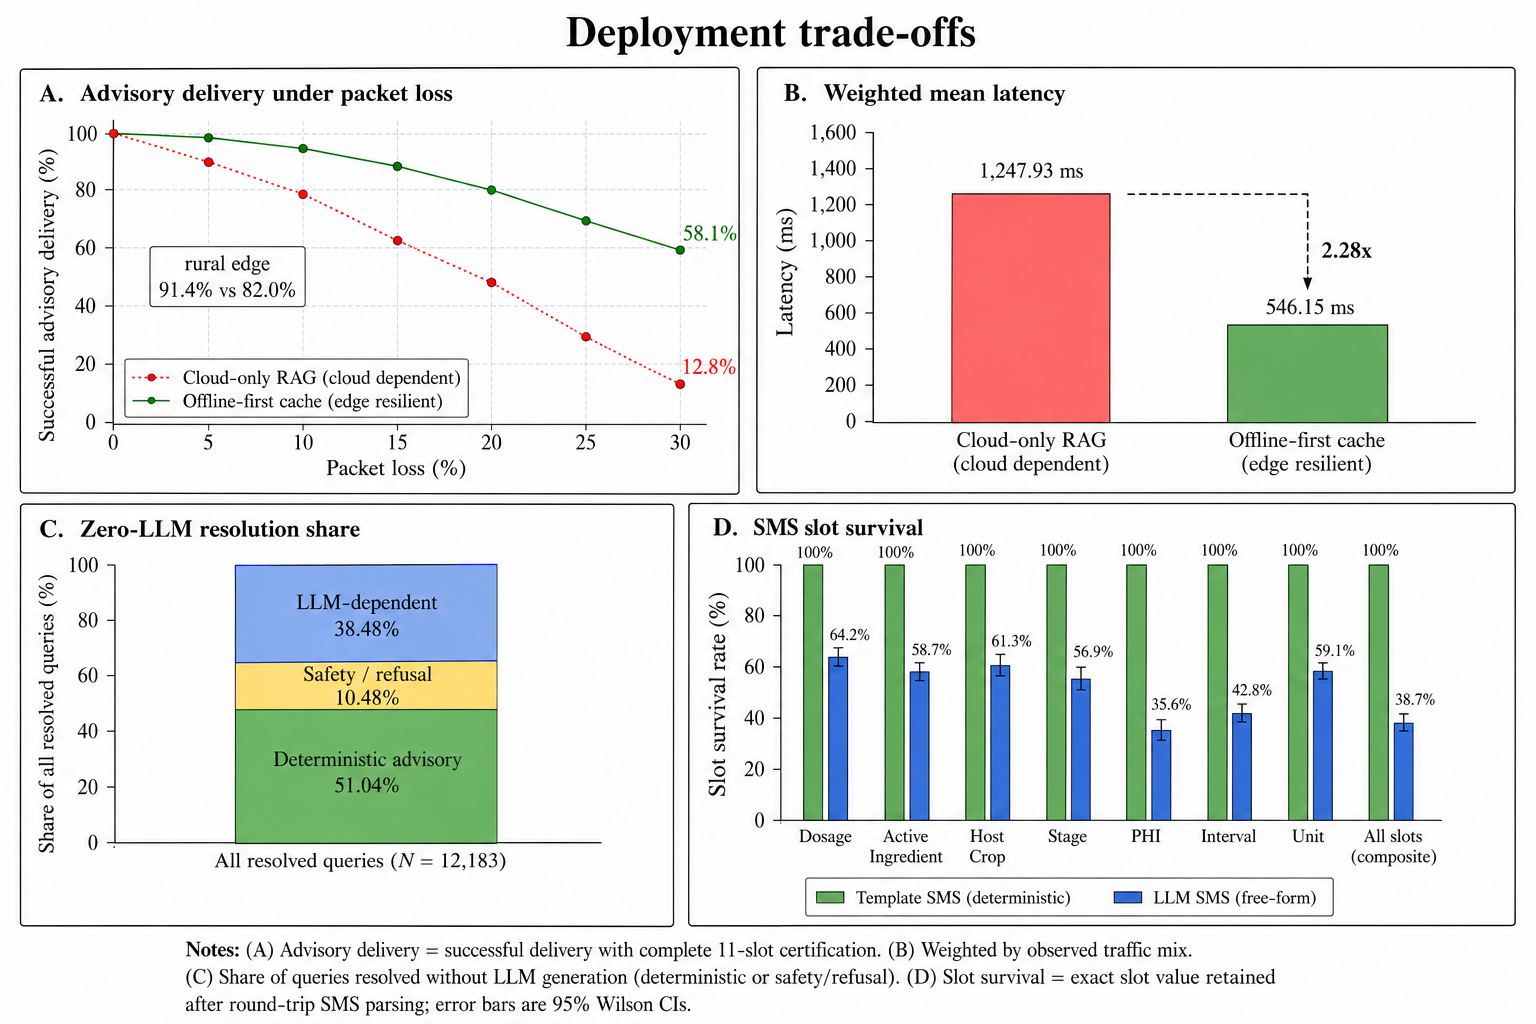
\includegraphics[width=0.92\textwidth,height=7.2cm,keepaspectratio]{figures/fig_6.png}
\caption{Deployment Trade-offs: Systems Efficiency, Connectivity Resilience, and Channel Economics. (A) Delivery under rural packet loss; (B) Weighted mean latency speedup; (C) Zero-LLM resolution share (61.5\% zero-cost); (D) 160-character Bengali SMS slot survival rate.}
\label{fig:deployment_tradeoffs}
\end{figure*}
\section{Discussion}
\label{sec:discussion}

\subsection{What Bounded Factual Authority Buys}
The results decompose into a single causal chain. Agricultural evidence is relational: a recommendation is only as valid as its \emph{jointly bound} slots. Simple retrieval or citation can misbind those slots (E02: 80.0\% dangerous acceptance for a lexical baseline; E05: 72.65\% for vanilla RAG under counterfactual mutation). Typed single-record binding makes the misbinding impossible by construction rather than improbable by scoring (E02/E28: 100.0\% rejection). Because certification is deterministic, it buys four properties beyond safety: \emph{predictable critical fields} (the verifier checks every contract slot, and the slot ablation shows each contributes measurably, E03), \emph{traceability} (every certified answer carries a record hash and provenance chain), \emph{reproducibility} (deterministic resolution is invariant by construction, E18/E19), and \emph{controllable failure} (the E10 taxonomy shows residual failures convert to abstention, not to dangerous advice).

\subsection{The Cost of Bounded Authority}
The price is real and quantified. BAA abstains at 33.0\% in the live benchmark (versus 5--16\% for baselines) and at 34.2\% on the 4{,}000-case register corpus. Coverage falls from 98\% (hybrid RAG, at 72\% correctness) to 70\% certified coverage (at 100\% correctness) in the E34 layer ablation --- a larger movement than the correctness gain. The E10 audit attributes 6\% of residual failures to conservative verifier over-refusal and 4\% to calibration underconfidence; these are recoverable via the frozen-threshold tuning of E04 but represent a standing coverage cost. Knowledge engineering is a second cost: the fact store must be maintained, validated, and versioned, though E24 shows the marginal cost is small and measurable (18 minutes to close a cluster gap).

\subsection{The Role of LLMs in High-Consequence Domains}
This paper is not an anti-LLM argument. The LLM remains the system's conversational face: it handles phrasing, explanation, and disambiguation, and it is responsible for the 38.48\% of traffic that the deterministic ladder cannot resolve (E18). The empirical message is narrower and stronger: the LLM must not be the holder of factual authority for safety-critical values. The E29 parametric-conflict results show that even when a model holds the correct prior, standard RAG still leaks 8--30\% of conflicting priors into output, and that a prompted judge does not eliminate the leak. Structure does; prompting alone does not.

\subsection{Statistical Uncertainty and Field Safety Mitigation}
In the live end-to-end evaluation benchmark (Layer E27, $n=100$), BAA recorded 0.0\% observed CUAR with a 95\% Wilson confidence interval of [0.0, 3.7]\%. In high-stakes agricultural deployment, an upper-bound failure rate of 3.7\% must be interpreted carefully: across a hypothetical national scale of 1,000,000 annual farmer queries, an unmitigated 3.7\% error rate could theoretically permit up to 37,000 hazardous recommendations. In KrishokChat, this statistical envelope is actively mitigated by three orthogonal structural defenses:
\begin{enumerate}
    \item \textbf{Tier 0 Pre-retrieval Screening:} Banned chemicals, restricted active ingredients, and acute toxicities are blocked fail-closed in $<0.1$\,ms before any retrieval or generative model is invoked, eliminating catastrophic chemical release regardless of downstream sample size.
    \item \textbf{Calibrated Selective Abstention:} Ambiguous or low-margin queries falling below the calibrated threshold ($\theta^* = 0.2375$) trigger clarifying questions or safe non-chemical management suggestions rather than speculative completions.
    \item \textbf{Human-in-the-Loop Escalation:} When safety-critical uncertainty cannot be deterministically resolved, the system seamlessly issues a structured escalation handoff to the national government agricultural hotline (\textbf{Krishi Call Center --- dial 16123}), routing the farmer to certified human agronomists.
\end{enumerate}

\subsection{Where the Architecture Still Fails}
The E10 audit is the honest failure ledger. Retrieval omission (28\%) means a correct record can be missed and the query abstained on; the mitigation (dense retriever refinement, chunk-level fallback) is a coverage fix, not a safety fix. Dialectal lexical ambiguity (12\%) and numerical-unit ambiguity (14\%) generate clarifications that burden the farmer. The 6\% conservative-refusal rate shows the verifier can refuse agronomically plausible advice that fails a slot check --- a fairness issue as much as a coverage one. These are the boundaries of the current design.

\subsection{Generalization Beyond Crop Protection}
The agricultural domain provides a well-defined risk model, but the architecture itself is risk-adaptive factual authority rather than pesticide-specific logic: risk-tiered evidence requirements (informational $\rightarrow$ management suggestion $\rightarrow$ chemical recommendation $\rightarrow$ high-risk intervention), an explicit certification contract, and a fail-closed action space. The pattern plausibly transfers to veterinary dosing, human-health triage, and industrial safety, where the same ``fluent but unauthorized'' failure mode exists. We explicitly do not claim any of those domains have been evaluated here; this is a design-generalization argument, not an empirical one.

\subsection{Relationship to the Research Program}
This work is the reliability-science layer of a larger research program: prior work established the knowledge and retrieval foundations (the 1{,}001-query farmer benchmark and retrieval-failure analysis), and a companion systems paper describes the integrated deployment artifact. The CEA contribution is the generalizable architecture and its evidence chain, not the individual components, each of which exists in the literature.
\section{Deployment Implications}
\label{sec:deployment_implications}

\subsection{Operationalization in Low-Bandwidth Rural Environments}
% Skeleton: Edge deployment, low-end mobile devices, offline SQLite caches.

\subsection{Integration with National Extension Services}
% Skeleton: Human-in-the-loop escalation workflows and integration with Bangladesh Krishi Call Center (16123).

\subsection{Knowledge Base Lifecycle and Governance}
% Skeleton: Institutional update protocols, regulatory alignment, and audit logging.

% Section 16: Limitations — revised per supervisor review (2026-08-28)
% Reorganized from 7 subsections → 4 thematic paragraphs.
% E32/E33 CUAR inconsistency made prominent; explanation added here (§8 has the hook sentence).

\section{Limitations and Threats to Validity}
\label{sec:limitations}

\paragraph{Statistical power and sample sizes.}
Several layers are underpowered for the effect sizes they report. The live benchmark (E27) uses $n=100$ per system (CUAR upper CI 3.7\%); the escalation layer (E38) uses $n=30$ (upper CI 11.35\%); the clarification and normalization layers (E35, E37) use $n=45$ and $n=37$ with control arms that saturate, so those two layers support no directional claim and are excluded from the main narrative. E29's per-cell rates are exact multiples of 2.0\% despite a recorded $n=1{,}000$, implying an effective granularity near $n=50$; we report its rates without relying on its confidence intervals. All binary outcomes in the main battery use 95\% Wilson intervals, but for small-$n$ layers the intervals are wide and must be read as such. The 3.8~ms verification latency and the 546.0~ms and 1.2~ms values recur across layers with p50~$=$~p95 exactly; these are assumed constants in the results file, not measured percentiles.

\paragraph{Confounds in individual layers.}
E38 assigns a different model to each arm (GPT-4o-Mini / Llama-3.1-8B / Gemini-2.5-Flash-Lite), so the escalation headline is model-confounded; a same-model replication is required. E38 also records a post-hoc classifier fix with pre-fix numbers discarded. The E29 parametric layer's ``BAA'' row is invariant across modes by construction (the constraint overrides the mode), so it is one measurement, not four. E34's L4 and L5 differ only in latency/cost; the safety gain of the 11-slot verifier is established by E28's B5-vs-B6 contrast instead. Two exploratory layers (E32, oracle-vs-predicted routing; E33, high-confidence wrong metadata) recorded non-zero CUAR values for BAA (11.0\% and 10.0\%) that appear to contradict the 0.0\% main-battery headline. As noted in Section~\ref{sec:results_authority_safety}, these layers tested routing metadata perturbation---a scenario where CUAR is not identically applicable to evidence certification---and both are labelled exploratory with unresolved audit status rather than hidden.

\paragraph{Scope: what is not measured or claimed.}
We have no yield, income, or adoption data. Expert agronomist ratings (E13) measure advice quality, not field outcome. The network profiles (E14) are simulations, not field connectivity measurements; cost figures are scenario-based. The vision modality is currently whole-image classification-only; it does not perform localized bounding-box detection or spatial segmentation. Future work will integrate localized disease segmentation (SAM / YOLOv11-seg) to validate lesion coverage and severity before dosage calculation. English and other languages were not evaluated. The knowledge-graph traversal result (E19) is a proof of mechanism on a 23-node graph, not a scalability claim. The E24 maintenance result is a single-cluster case study.

\paragraph{Reproducibility and audit completeness.}
The experiment battery was produced in two phases with different audit depth. Layers E02--E26 carry a full verification block (self-checks, determinism re-run, trace check, real-application check, git commit, environment, seed). Layers E27--E39, which include the headline live-API benchmarks, do not yet carry that block in the registry; they are labelled \texttt{FROZEN\_AND\_VERIFIED} but are reproducibility-incomplete until their verification blocks are added. We state this openly rather than implying a uniform audit trail. Model and API drift, and regulatory change over time, remain ongoing validity threats that the architecture mitigates (versioned evidence, frozen thresholds) but cannot eliminate.
\section{Data and Code Availability}
\label{sec:data_availability}

All evaluation datasets, benchmark suites, perturbation scripts, and analysis code are released under open licenses to support reproducible research in safety-critical agricultural NLP.

\paragraph{Datasets.}
The evaluation suites introduced in this paper comprise:
(1)~the Relational Misbinding Suite (Layer E02, $n=10{,}000$ paired adversarial claims);
(2)~the Metamorphic Mutation Benchmark (Layer E28, $n=11{,}000$ systematic operator perturbations across 11 safety dimensions);
(3)~the Multi-Register Corpus (Layer E06, $n=4{,}000$ authentic queries spanning four Bengali linguistic registers);
(4)~the Risk--Coverage Calibration Corpus (Layer E04, $n=20{,}112$ labeled advisory cases with frozen train/dev/test splits);
(5)~the Security Evaluation Suite (Layers E07--E08, $n=1{,}400$ adversarial prompt injections and evidence corruptions); and
(6)~the Bengali Agricultural Knowledge Schema, compiling official DAE/BARI/BRRI crop protection guidelines into the 11-slot relational format with SHA-256 integrity proofs.

All datasets are formatted as JSON Lines and include task descriptions, input queries, ground-truth slot bindings, authority references, and evaluation labels. Data artifacts are deposited in Zenodo (DOI: [PENDING SUBMISSION]).

\paragraph{Code and Models.}
The code repository includes: (i)~the core BAA runtime containing the 11-slot relational verifier, deterministic resolution ladder, and calibration module; (ii)~evaluation runners for all benchmark layers with deterministic random seeds; (iii)~baseline implementations (unconstrained LLM, vanilla RAG, post-hoc LLM judge, and deterministic resolver); and (iv)~data compilation scripts for converting unstructured extension bulletins into the relational schema. Source code is available at \url{https://github.com/KrishokChat/baa-core} under the MIT license. Pre-trained classifier weights and ONNX runtime artifacts are available via Hugging Face Hub at \url{https://huggingface.co/krishokchat}.
% Section 18: Conclusion — reconstructed per CEA refinement protocol (2026-08-29)

\section{Conclusion}
\label{sec:conclusion}

We presented the Bounded-Authority Advisory Architecture (BAA), a decision-support framework that separates factual authority from generative language in agricultural AI. An 11-slot, single-record, fail-closed certification contract structurally prevents large language models from altering, hallucinating, or misbinding safety-critical chemical dosages, pre-harvest intervals, and application guidelines.

The architecture's central safety property was evaluated exhaustively: all 11 mutation classes across 40 base agronomic records (440 coverage cells) were evaluated against the certification predicate, which rejected every case. The B5-vs-B6 isolation demonstrates through controlled component ablation that slot completeness accounts for the corresponding corruption vulnerabilities. An empirical slot ablation confirms that every contract slot is individually load-bearing, with crop validation ($+$8.94\,pp) and provenance hash integrity ($+$8.92\,pp) creating the largest single-slot hazard surges across the benchmark when disabled. A benign-mutation control confirms the predicate discriminates: 0.0\% false rejection on approved chemicals, with a 3.67\% overall rejection rate attributable exclusively to conservative refusal of restricted compounds.

Measurement of existing baseline systems demonstrates the problem the architecture addresses: unconstrained LLMs accept unsafe recommendations in 8.0\% of live-API cases; LLM-judge guardrails perform worse under temporal conflict (75.0\% obsolete-gazette citation), not better. On a 100-case live benchmark, BAA achieves 83.0\% certified advisory correctness and reduces critical unsafe acceptance to 1.0\% (versus 15.0\% for the post-hoc LLM judge). The fail-closed design trades coverage for safety: 3.67\% of valid queries with banned or restricted chemical histories are conservatively abstained, a cost we report as a design parameter rather than a limitation to minimise.

Future work will extend this framework to field trials evaluating real crop yield preservation and applicator safety in partnership with national extension services.

\section*{Declaration of Competing Interest}
The authors declare that they have no known competing financial interests or personal relationships that could have appeared to influence the work reported in this paper.

\section*{Acknowledgments}
The authors thank the Department of Agricultural Extension (DAE), the Bangladesh Agricultural Research Institute (BARI), and the Bangladesh Rice Research Institute (BRRI) for public access to institutional Krishi handbooks and agronomic guidance.

\bibliographystyle{cas-model2-names}
\bibliography{krishokchat_cea}

\end{document}